\documentclass[10pt,a4paper]{book}
\usepackage[english]{babel}
\usepackage[T1]{fontenc}
\usepackage[utf8x]{inputenc}
%\usepackage{fancyhdr}
%\pagestyle{fancy}

\usepackage{amsmath}
\usepackage{amssymb}
\usepackage{mathrsfs}
\usepackage{amsfonts}
\usepackage{amsthm}
\usepackage{mathtools}

\usepackage{paralist}

\usepackage{scrextend}
\addtokomafont{labelinglabel}{\sffamily}

\usepackage{cases}

\usepackage[colorlinks]{hyperref}
\hypersetup{hidelinks}

\theoremstyle{definition}
\newtheorem{defin}{Definition}[chapter]
\newtheorem{prop}[defin]{Proposition}
\newtheorem{theorem}[defin]{Theorem}

\DeclareMathAlphabet\mathbfcal{OMS}{cmsy}{b}{n}
\usepackage{mymacrosTESI}

\usepackage{graphicx}
\usepackage[margin=10pt,font=small,labelfont=bf]{caption}
\usepackage[labelfont=bf,list=true]{subcaption}
\graphicspath{ {Figure/} }

\usepackage{booktabs}

\usepackage[titletoc,page]{appendix}

\usepackage{algorithmicx}
\usepackage[chapter]{algorithm}
\usepackage{algpseudocode}

\usepackage{pdfpages}

\newcommand{\lr}[1]{\textcolor[rgb]{0.8,0,0}{LR: \textbf{\textit{#1}}}}


\begin{document}

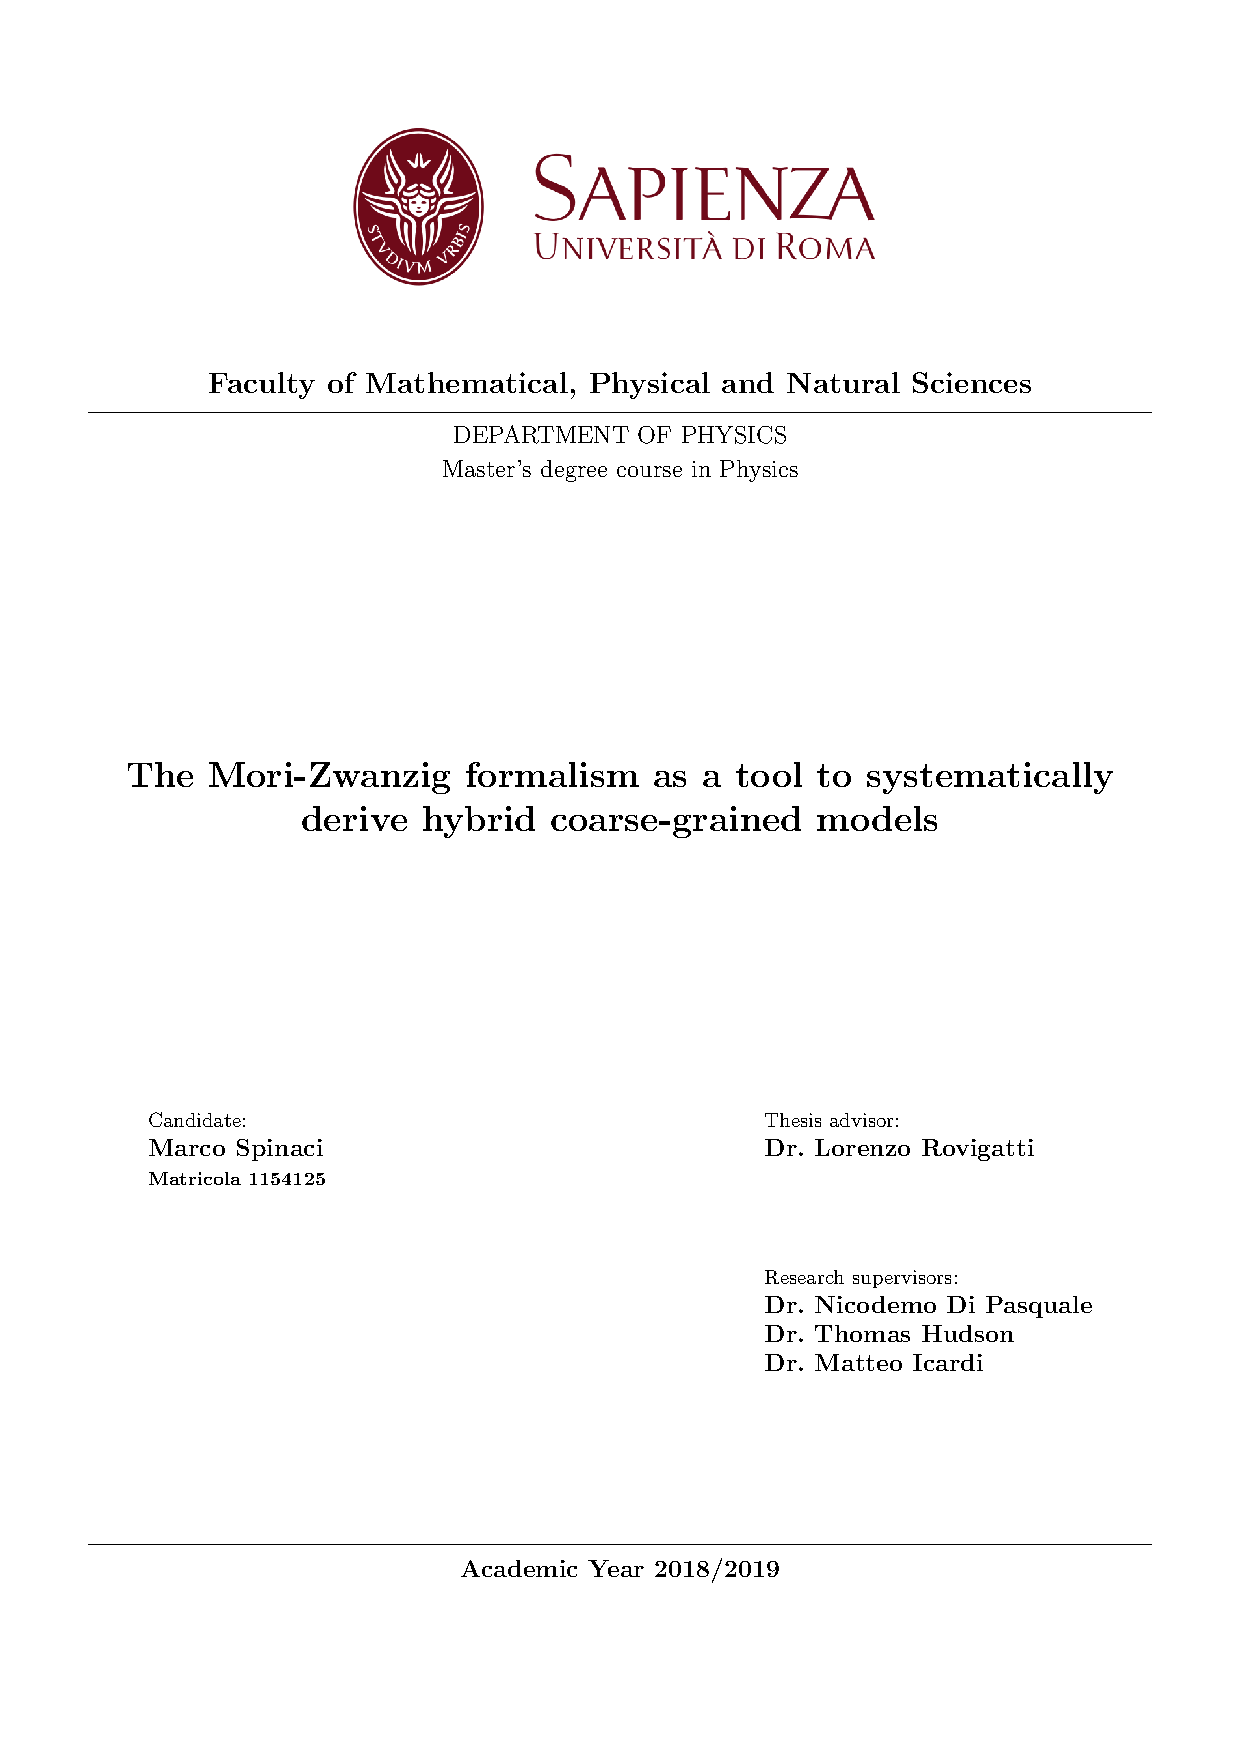
\includepdf{Front.pdf}

\frontmatter

 
\begin{center}
\section*{Abstract}
\end{center}

My Master thesis project deals with the Mori-Zwanzig (MZ) formalism as a tool to systematically derive hybrid coarse-grained (CG) models. The MZ formalism allows to study the evolution of a dynamical system through the projection on a subset of its degrees of freedom. This operation can be done through various projection operator techniques \cite{Grabert:Projection}. 
%
The project builds on the work of N. Di Pasquale \emph{et al.}~\cite{DiPasquale2019}, in which the authors derived a coarse-grained model for hybrid systems through the MZ projection, with a theoretical discussion supported by numerical simulations limited to the microcanonical (NVE) ensemble.
%


The first part of the thesis focusses on the derivation of the equations governing the coarse-grained dynamics, obtained through the MZ formalism.
The equations of motion obtained are described by a Generalized Langevin Equation (GLE), which is an equation that allows to describe a particle, in a system in or close to equilibrium, subject to a potential and coupled to a general thermal bath in which memory effects are, in general, present.

The second part of the thesis is focused on the study of numerical methods for Langevin dynamics and for the constrained Langevin dynamics. These methods are used to numerically implement the full and the constrained dynamics in the canonical (NVT) ensemble. The integrators we choose to integrate the equations of motions have been developed by Leimkuhler \emph{et al.} \cite{LeimMatt:LAnDynInt,Leimkuhler2016}. These methods are splitting integrators that decompose the stochastic vector field which drives the Langevin Dynamics into simpler vector fields which can be solved exactly. In particular, we used the BAOAB method to sample the full dynamics\cite{LeimMatt:LAnDynInt}, and the geodesic-BAOAB method to to sample the constrained dynamics \cite{Leimkuhler2016}.

The third and final part of the thesis is on the numerical experiments in the canonical (NVT) ensemble by extending and improving the open-source parallel code, written in Julia 0.6, developed by Di Pasquale \emph{et al.} \cite{DiPasquale2019}, introducing the integrators studied in the previous part. This code allows to solve the full, constrained and coarse-grained dynamics, as well as all the components needed for the coarse-grained (CG) system.
%
The full-resolution (fine-grained, FG) system that we consider is a periodic chain of $\nfg$ ``atoms'' of two different species, which are assumed to have different masses and bond stiffness, in a repeating pattern. We assumed that the chemical structure of the molecular system is fixed, \textit{i.e.} no reactions occur. Each ``atom'' is mapped to a fixed (unique) particle in the CG system, called bead. 
We performed the simulation for four different systems with different parameter and for different dynamics: the FG dynamics, the orthogonal dynamics (or constrained dynamics), the coarse-grained dynamics and the Markovian Mori-Zwanzig dynamics.


\tableofcontents

\mainmatter

\chapter*{Introduction}
\phantomsection
\addcontentsline{toc}{chapter}{Introduction}
\markboth{\MakeUppercase{Introduction}}{\MakeUppercase{Introduction}}

Molecular Dynamics (MD) is a computational approach that allows to solve the equations of motion of a system of atoms, and to compute the macroscopic observables from the generated trajectories, while at the same time allowing the detailed visualization of the movements of the individual atoms in the system under examination, providing a ``window'' into the microscopic world \cite{tuckerman2010}. The question that arises is relative to the interpretation of MD simulations, that is, consider them realistic, or interpret them as useful tools to guide us toward an understanding of the mechanism underlying a given chemical process.
%
Klaus Schulten, whose research group developed highly popular molecular dynamics software packages such as NAMD and visualization software such as VMD, had a strong opinion on the matter. In fact, in his 2015 National Lecture \cite{Pollack}, he introduced the term ``computational microscope'' to describe the role of computational simulations in the study of biological systems. He believed that computational biophysics has progressed to the point that it provides a realistic view of the biological cellular components at the molecular level, often at a resolution not achievable through laboratory instruments, reaching atomic or even electronic dimensions.  
``The point I wanted to make,'' said Klaus Schulten about the National Lecture, ``is that basically molecular modelling came of age, and it's now a full member of the scientific community in the sense that we can play the most glorious and important part of science, namely to make discoveries.'' 

Despite recent advances in simulation methods, atomistically detailed models and computational resources, MD simulations are heavily limited in terms of system size and simulation time. For example, most biomolecular events of interest, such as protein folding or major conformational changes essential for protein function, occur on time scales longer (from microseconds to milliseconds) than time scales accessible to MD simulations  \cite{Aminpour2019,Freddolino2008}.
In fact, remarkable recent atomistic simulations are represented by the folding studies of small proteins of Schulten \textit{et al.}~\cite{Freddolino2008} and Shaw \textit{et al.}~\cite{Shaw2010}. The Schulten group achieved a continuous trajectory of $10\, \mu s$ while the Shaw group performed a $1\, ms$ long simulation. Despite these successes, atomistic simulations are still several order of away magnitude far from being able to effectively cover the time and length scales of most cellular processes.
%
For an idea of time scales and length scales, as well as the time-line of progress in the system size accessible to all-atom MD simulations up to 2014, see fig.~\ref{Fig:sketchResolution} and fig.~\ref{Fig:evolutionSize}, respectively.
%
\begin{figure}[htb!]
 \centering
 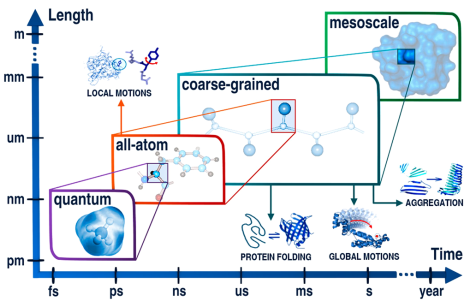
\includegraphics[width=0.8\textwidth]{RangesMD}
 \caption{Sketch of the application ranges for molecular modelling at different resolutions: quantum, all-atoms, coarse-grained and mesoscale. The plot 
shows approximate ranges of time scales and length scales  for the different resolutions of a generic system, as well as the approximate time and length scales of some biomolecular events of interest. Figure taken from Ref.~\cite{Kmiecik2016}. }
 \label{Fig:sketchResolution}
\end{figure}
%
\begin{figure}[htb!]
 \centering
 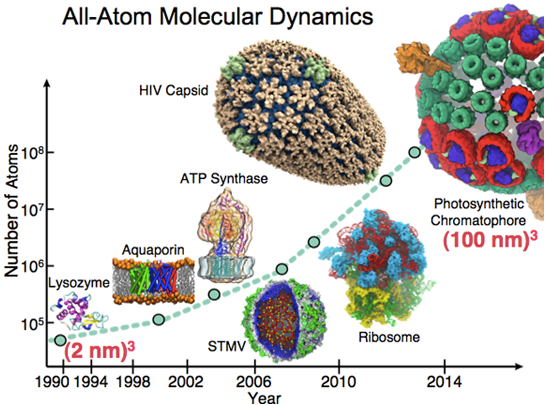
\includegraphics[width=0.8\textwidth]{EvolutionSize}
 \caption{Sketch of the time-line of progress in the system size accessible to all-atom MD simulations up to 2014. Figure taken from Ref.~\cite{Pollack}.}
 \label{Fig:evolutionSize}
\end{figure}

These limitations are given by the fact that in order to compute the equations of motion we have to provide as input the complete set of interatomic forces. The accuracy of these forces is of vital importance in order to have a reliable model of a complex system and unfortunately, as a general rule, the more accurate the forces are, the longer is the time needed to calculate them during the simulations.
%
Another problem often encountered in \textit{in silico} investigations of long chain-like molecules is that the relaxation time required to approach equilibrium becomes comparable with the currently accessible simulation time scales, as the size of the system increases \cite{Maginn2009}. 

However, MD simulations have become a standard tool in many areas of research, for example in soft matter \cite{Corezzi2008,Klein2008,Peter2009} as well as in the study of biological systems \cite{KLEPEIS2009}, and are often used in combination with a wide variety of experimental techniques \cite{HOLLINGSWORTH2018,Spagnolli2019}. 

Various methods have been introduced to overcome these limitations, including the \emph{coarse-grained method} (CG) and the so-called \emph{enhanced sampling methods}. The former simplifies and accelerates MD simulations \cite{Brini2013}, by grouping atoms of the atomistic model under examination and treating these groups as individual sites of interaction. This idea was introduced by Levitt and Warshel in the 1970s \cite{Levitt1975,Levitt1976}. 
The latters only address the problem of the time scale and include methods like Umbrella sampling \cite{Kumar1992,TORRIE1977}, Steered molecular dynamics \cite{ISRALEWITZ2001,SMDbook1999} and Metadynamics \cite{Laio2002}. 
In this work we will not deal with the enhanced sampling methods but we will present a full derivation of a generic CG model through the Mori-Zwanzig (MZ) formalism \cite{DiPasquale2019,Hijon2010}.

As we mentioned above, in the CG models the fundamental particles are interaction sites (sometimes called beads) that represent group of atoms, and comprise typically on the order of 2-10 ``heavy'' atoms (\textit{e.g.}, C, N, O, P) and their associated hydrogen atoms \cite{Noid2013Book}.
The procedure for transforming an atomically detailed structure into a coarse-grained representation of the same structure is called \emph{CG mapping}.  Of course, the mapping can be customized to accurately capture the key characteristics of a specific system or phenomenon of interest, while eliminating atomic details that are considered ``unimportant''. 
The construction of the mapping is the first step in defining a CG model, and it is intimately related to its accuracy, efficiency and transferability\footnote{``Transferability'' means the property of a CG mapping to hold under a change of conditions, such as temperature, density, concentration, system composition, phase, \textit{etc.}~of the system under consideration, as well as a change in the chemical environment, \textit{e.g.}, a change in the length or sequence of an amino acid chain \cite{Potestio2014}.}. In particular, the accuracy and transferability of a CG model do not necessarily increase as the resolution of the system mapping increases \cite{Mullimax2009,Potestio2014}. In fig.~\ref{Fig:CGpictureMM} we show a sketch of the CG mapping of a peptdide, \textit{i.e.}, a short chains of amino acids linked by peptide bonds.
\begin{figure}[htb]
    \centering
    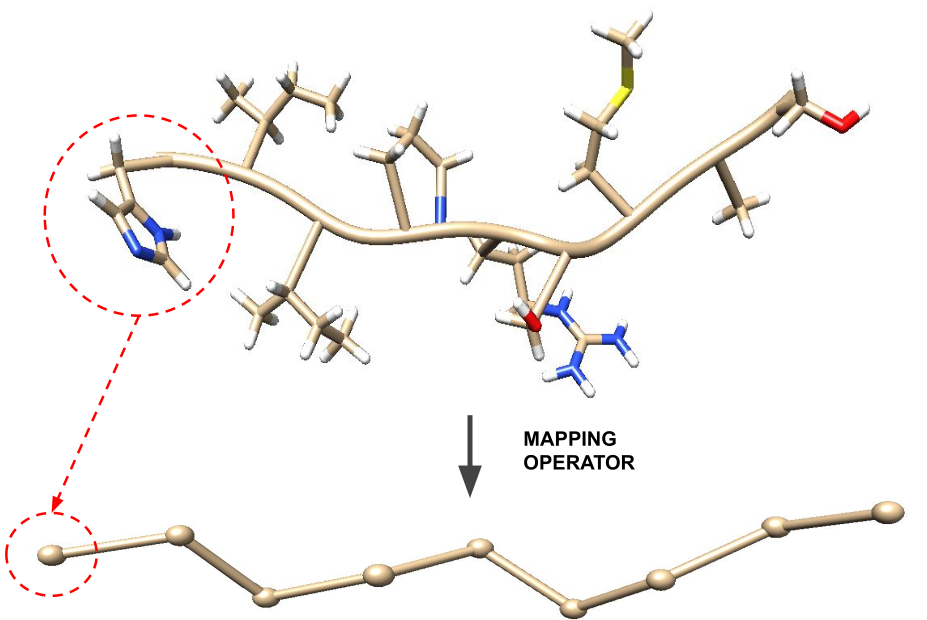
\includegraphics[width=0.9\textwidth]{CGmm.png}
    \caption{Sketch of the coarse-grained mapping of a peptdide (\textit{i.e.}, a short chain of amino acids linked by peptide bonds), made with UCSF Chimera, developed by the Resource for Biocomputing, Visualization, and Informatics at the University of California, San Francisco, with support from NIH P41-GM103311 \cite{Chimera2004}.}
    \label{Fig:CGpictureMM}
\end{figure}

Once the representation of the CG model has been determined, the new challenge is to determine an appropriate interaction between the CG sites (\textit{i.e.}, between the beads). These interactions are described by \emph{effective potentials} that should take into account the effects of the atomic details that have been eliminated from the CG model. For example, in the implicit solvent CG models, all solvent molecules are formally integrated out and their effects are incorporated into the interactions between the remaining sites \cite{Silbermann2006}.
Therefore, the interactions in the CG model should reflect the ``correct physics'' so that the model, in addition to being highly efficient, ideally provides both fundamental insights and quantitatively accurate predictions. 
%
Generally, two types of approach are used to determine the interaction between beads, the \emph{bottom-up} approach (structure-based coarse-graining) and the \emph{top-down} approach (thermodynamic-based coarse-graining).

\noindent
A \emph{bottom-up} CG model is a model of a particular system that is constructed on the basis of a more detailed model of the same system, and consequently the effective potential is parameterized on the basis of comparisons with atomistic reference simulations. Various methods can be used to do this, the most commonly used being the inverse Monte Carlo (IMC) \cite{Lyubartsev1995}, the iterative Boltzmann inversion (IBI) \cite{Reith2003}, force matching (FM) \cite{Izvekov2004,Izvekov2005,Noid2008} and minimization of relative entropy \cite{Chaimovich2011}.
%
\emph{Top-down} models, instead, are not based on or refer directly to more detailed descriptions of the particular system studied, but may be parameterized on the basis of experimental data, in particular thermodynamic data, such as solvation free energies and partitioning data, liquid densities, surface tension, \textit{etc.}~\cite{CLEMENTI2008,Honeycutt1990,Nielsen2003}.

\noindent
There is a second common distinction for CG models of biomolecular systems, which distinguishes CG models between \emph{physics-based} and \emph{knowledge-based} approaches. The former use physical theories to deduce interactions in CG models, and comprise the approaches described above, \textit{i.e.} the \emph{bottom-up} approach and the \emph{top-down} approach. By contrast, the latter are constructed on the basis of information extracted from experimentally determined three-dimensional structures.
In fig.~\ref{Fig:CGStrategies} the distinctions between the various approaches are shown in a schematic way. 

\vspace{0.1cm}
Typically, CG simulations can be three or four orders of magnitude more efficient than all-atom simulations for several reasons:
\begin{enumerate}[(i)]
\item CG models require fewer interacting sites to model the same system, so fewer interactions must be calculated at each time step;
\item interactions in CG models are typically short-range compared to interactions in atomistic models. For example, long-range Coulombic interactions may be examined more effectively on the length scales relevant for CG interactions and can be modelled as short-range effective potentials \cite{Noid2013Book,Silbermann2006};
\item effective potentials can implicitly include entropic effects and greatly reduce the need to explicitly sample a large number of degenerate atomically detailed configurations \cite{Levitt1975};
\item interactions between CG sites are usually ``softer'', (\textit{i.e.}, of lower frequency) which allows a larger integration time step for propagating dynamics \cite{Marrink2004}. In other words, we are saying that the fluctuations of the force that CG sites experience are generally smaller, leading to a smoother free energy profile \cite{Rudzinski2019}. As a result, we have a faster diffusive process allowing the system to reach greater time scales with fewer computations. This last aspect implies that one typically has to determine a rescaling factor between the simulation timescale (usually given in Lennard Jones units) and the corresponding timescale in all-atom system (or the corresponding real world time \cite{Fritz2011,Potestio2014}.
\end{enumerate}

\begin{figure}[htb]
    \centering
    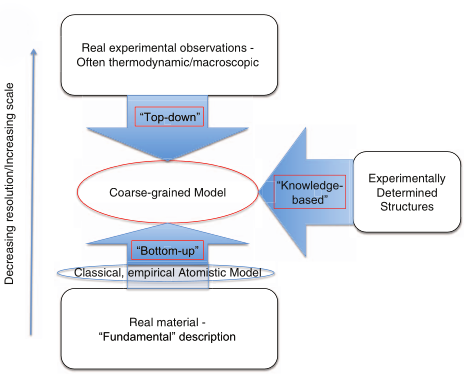
\includegraphics[width=0.9\textwidth]{CGStrategies}
    \caption{Sketch with strategies for CG distinguishing between top-down, bottom-up, and knowledge-based approaches. Figure taken from the Ref.~\cite{Noid2013}.}
    \label{Fig:CGStrategies}
\end{figure}

If we are interested in the dynamic properties of the system under consideration, what has been said in the last point is one of the main limits of most CG models. This difference in time scales between two resolution levels of the same system does not allow to preserve the dynamic properties. This artificial acceleration of the dynamics could be corrected by adding appropriate friction terms in order to obtain a better estimate of the dynamic observables \cite{Izvekov2006}. 

A second limitation of coarse-grained models is the loss of information about the model caused by CG mapping. In fact, some phenomena such as hydrogen bonds are only observable at the atomistic level. These phenomena need special treatment to be considered in a CG model \cite{Karimi-Varzaneh2008}. These limitations have led to the development of \emph{hybrid} atomistic/CG models that ideally should combine both a lower computational cost than all-atom simulations and greater accuracy than CG simulations \cite{DiPasquale2012,Rzepiela2011}.
However, even these models, when considering the dynamics, have some problems. For instance, it has been shown that considering complex systems such as polymers new effects arise \cite{DiPasquale2017}. Therefore, a rigorous treatment of these models becomes necessary.

As mentioned above, the CG approach studied here is the Mori-Zwanzig projection formalism \cite{Mori1965,Zwanzig1973}. One of the first applications of this formalism to obtain CG models was made by Givon et al. \cite{Givon2004}. This formalism, given an arbitrary and generic CG mapping, allows a rigorous derivation of the equations for the exact evolution of CG variables, including terms that may be identified as a term of friction with a memory kernel and a fluctuating force, consistent with the fluctuation-dissipation theorem. Moreover, under the assumptions made to derive the equations, it provides an explicit and rigorous means by which to compute the CG interactions and a framework in which to improve and quantify the accuracy \cite{DiPasquale2019}.
Despite the explicit form of the terms appearing in the CG equations of motion derived through MZ formalism, these terms are not easy to compute. In recent years, significant efforts have been made to solve these problems and make CG simulations more practicable using this theoretical tool \cite{DiPasquale2019,Espanol2009,Hijon2010,Izvekov2017,Jung2017,Li2015,Wang2019,Yuanran2018}.

%The thesis is organized as follows: $\dots$ to be continued $\dots$


\part{Theoretical Background}

\chapter{Mori-Zwanzig Formalism}
The Mori-Zwanzig formalism allows to study the evolution of a dynamical system through the projection on a subset of its degrees of freedom. This operation is done through \emph{projection operator techniques}.

The \emph{projection operator technique} is a collection of powerful tools for the study of irreversible processes in many-body systems \cite{Grabert:Projection}. These tools were introduced into statistical physics by S. Nakajima in 1958 \cite{Nakajima1958} and R. Zwanzig in 1960 \cite{Zwanzig1960}. The former used them to study the quantum statistical mechanics of steady diffusion, while the latter to give a new formulation of methods introduced in the statistical-mechanical theory of irreversibility. In particular, R. Zwanzig developed the technique into a tool for deriving formally accurate equations of motion for classical or quantum probability densities \cite{Zwanzig1961,Zwanzig1964}. Later in 1965, H. Mori proposed a different framework, which leads to the following linear \emph{generalized Langevin equation} (GLE)
\begin{equation}\label{generalGLE}
 \frac{\diff A}{\diff t}=i\Omega A(t)-\int_0^t\,\diff\tau K(\tau)A(t-\tau)+F(t)\,,
\end{equation}
where $\Omega$, $K(t)$ and $F(t)$ are called frequency, memory function and random force, respectively.
This equation describes the non-equilibrium evolution of any set of functions $A(t)$ defined on the phase-space of the arbitrary microscopic system, close to thermal equilibrium \cite{Mori1965}. These variables $A(t)$ are called collective variables, relevant variables, coarse-grained (CG) variables or collective modes, depending on the context.

\noindent
Some years later in 1973 R. Zwanzig derived a class of generalized Langevin equations describing the motion of a system interacting with a heat bath. This GLE is exact but differs from that obtained by Mori's scheme for two reasons: for the presence of an arbitrary nonlinear force and for the fact that its validity is not restricted to small deviations from the thermal equilibrium \cite{Zwanzig1973}.

\noindent
In recent years D. Kauzlari\'c \textit{et al.}~\cite{Kauzlaric2011} showed in their work on the calculation of the friction matrix in the coarse-grained description of an atomistic system that Mori's GLE can be obtained from the Zwanzig's one if the system is close to the equilibrium and under the Markovian assumption, i.e. that the relevant variables (the functions $A(t)$ in the eq.~(\ref{generalGLE})) have a characteristic time scale much larger than the memory time scale.

These techniques are known in various context as well as in transport theory. For example, in the dynamic light scattering or in the liquids theory, the GLE is used to compute time-correlation functions under circumstances where the usual phenomenological equations do not apply. Indeed, the Mori-Zwanzig formalism can be used to obtain an equation for the time correlation function $C(t)$:  
\begin{equation}
 \frac{\diff C(t)}{\diff t}=i\Omega\, C(t)-\int_0^t\,\diff\tau K(\tau)C(t-\tau)\,.
\end{equation}
This equation can be derived from the equation (\ref{generalGLE}), is called the \emph{memory-function equation} and the random force appears implicitly in $K(t)$ \cite{Berne:DynamicLightScatt,hansen2006}.

If the dynamical system considered is Hamiltonian, in the Mori-Zwanzig formalism we can use two equivalent approaches:
\begin{enumerate}[(i)]
  \item applying the projection operator in a Hilbert space of probability densities function (pdf) to the Liouville equation, obtaining the generalized Fokker-Planck and master equations \cite{Kinjo2007,Zwanzig1960,Zwanzig1961,Zwanzig1964};
  \item applying the projection operator in the Liouville space (see appendix \ref{App:C}) to the equation of motion of time-dependent phase-space function, obtaining the GLE and the transport equation \cite{DiPasquale2019,Hijon2010,Mori1965,Nordholm1975,Zwanzig1973}.
\end{enumerate}
The mathematical equivalence of these two approaches is given by the duality between Liouville space and the space of densities of states, in complete analogy with the Schr\"odinger and Heisenberg pictures in Quantum Mechanics. 

\noindent
In what follows, we choose to follow the second approach since this results in a more physically-intuitive derivation.
Here, we will derive the GLE for the CG variables through the \emph{Zwanzig projection}. We will not give a derivation of the eq.~(\ref{generalGLE}) since it can be found in various books (see Ref.~\cite{Berne:DynamicLightScatt,evans2008,hansen2006,tuckerman2010}) and is similar to the one that we will show through the \emph{Zwanzig projection}.

We assume that, at the microscopic level, the system is well described by classical mechanics and is composed by $\nfg$ particles. We will refer to it as the \emph{fine-grained} (FG) system. The microscopic state is characterised by the function $\Aphase{}(t)$ in a $6\nfg$-dimensional phase-space. 

\noindent
To derive a reduced description of this system, we consider a smaller set of phase function $\Bphase{}(\Aphase{})$, which we call \emph{observables}\footnote{
Throughout the present section, these observables could be quite general, but we will later apply the derivation made here to a particular choice.
}.
The time evolution of a function of phase variables is given by
\begin{equation}\label{Eq:MotionEqGamma}
  \totd{\Bphase{}(\Aphase{}(t))}{t} = \Lio\,\Bphase{}(\Aphase{}(t))\,,
  \quad\Bphase{}(\Aphase{}(0)) \equiv \Bphase{}(\Aphase{0})\,.
\end{equation}
Here, the operator $\Lio\equiv iL$ is the \emph{Liouvillian} (see appendix \ref{App:C}) and the formal solution is given by
\begin{equation}\label{Eq:SolLiouville}
	\Bphase{}(\Aphase{}(t)) = \exp{\Lio t}\,\Bphase{}(\Aphase{0})\,,
\end{equation}
where the exponential operator is defined through its Taylor expansion.
This solution implicitly depends upon the full evolution of the FG system, therefore this equation does not provide a self-consistent evolution equation for the observables. 

We also assume that the state of the system is described by the canonical equilibrium distribution\footnote{Different choices are possible. For example it is also perfectly possible to carry out the same derivation using the micro-canonical equilibrium measure.} $\rho^{eq}(\Aphase{})$, so that the probability equilibrium measure is given by the Gibbs measure on the FG phase-space $X=\real^{6\nfg}$:
\begin{equation}\label{Eq:GibbsMeas}
 \mathbb{P}(\diff\Aphase{})=\rho^{eq}(\Aphase{})\diff\Aphase{}=\frac{1}{\partf}\exp{-\beta\Ham(\Aphase{})}\diff\Aphase{}\,.
% \qquad X=\real^{6\nfg}\,;
\end{equation}

The Mori-Zwanzig formalism allows us to replace equation (\ref{Eq:MotionEqGamma}) for the observables $\Bphase{}(\Aphase{})$ by an equation of motion which depends on the microstate $\Aphase{}$ only through the CG variables themselves, but as we will see in the Sec.~\ref{Sec:GLE} the complexity of the computation of eq.~(\ref{Eq:MotionEqGamma}) will be shifted to the computation of the so-called \emph{orthogonal dynamics}.

%For example, with the \emph{Zwanzig projection} this is done by projecting the equation for the observables $\Bphase{}(\Aphase{})$ onto the space of functions of the CG variables, which may be regarded as a subspace of the FG observable space\footnote{This is true as long as some very broad measurability assumptions on the CG variables chosen are met; in practice, choosing CG variables which are continuous and differentiable in the FG variables is already sufficient, and this particular choice is implicitly assumed in the derivation presented here. In theory however, much more general choices can be made.}.


\section{Zwanzig approach}
\subsection{The Zwanzig Projection}
We denote the \emph{Zwanzig projection} as $\mathcal{P}_{\Bphase{}}$:
\begin{equation}\label{Eq:proj}
	\mathcal{P}_{\Bphase{}}F(\Aphase{}) = \frac{1}{\Omega(\Bphase{})} \int_X F(\Aphase{}')\,\dirac{\Bphase{}(\Aphase{}')-\Bphase{}}\rho^{eq}(\Aphase{}')\diff\Aphase{}'
\end{equation}
where $F(\Aphase{})$ is a generic function acting on the space-phase $X=\real^{6\nfg}$, $\Bphase{}$ is a smaller set of phase function (which we called observables) and the normalisation factor, also called the \textit{structure function}, represents the total volume of the surface $S(\Bphase{})$ in phace-space, which is defined by $\Bphase{}(\Aphase{}')=\Bphase{}$:
%
\begin{equation}\label{eq:structurefunc}
	\Omega(\Bphase{}) = \int_X\dirac{\Bphase{}(\Aphase{}')-\Bphase{}}\mathbb{P}(\diff\Aphase{}')\,.
\end{equation}
In other words, the \textit{structure function} represents the number of micro-states compatible with the macro-state $\Bphase{}(\Aphase{}')=\Bphase{}$ \cite{Hijon2010}, and the projection operator $\mathcal{P}_{\Bphase{}}$ selects from an arbitrary function $F(\Aphase{})$ the part, $\mathcal{P}_{\Bphase{}}F(\Aphase{})$, which depends on $\Aphase{}$ only through $\Bphase{}$.

\noindent
If we introduce a set of fixed values $\bfa$ such that for a given $\Aphase{}$ we have $\Bphase{}=\bfa$. The integral in the numerator represents the amount of $F(\Aphase{})$ contained in the correspondent surface $S(\bfa)$, while the \textit{structure function} in the denominator $\Omega(\Bphase{})=\Omega(\bfa)$ allows us to spread this amount on the surface $S(\bfa)$.
Therefore, loosely speaking, $\mathcal{P}_{\Bphase{}}$ ``averages'' the function $F(\Aphase{})$ over the surface $S(\bfa)$ in case the observables $\Bphase{}$ are equal to $\bfa$ for a given $\Aphase{}$.

The fact that $\mathcal{P}_{\Bphase{}}$ is a projection operator can be easily verified by showing that it satisfies the necessary and
sufficient conditions for a projection operator, \textit{i.e.}, it is Hermitian and $\mathcal{P}_{\Bphase{}}^2=\mathcal{P}_{\Bphase{}}$ \cite{Zwanzig1961}.
So we can define the \emph{complementary orthogonal projection} $\qproj_{\Bphase{}}$ as
$$
 \qproj_{\Bphase{}}=\idproj-\pproj_{\Bphase{}}\,,
$$  
where $\idproj$ is the identity operator.


\subsection{Zwanzig Projection as Conditional Expectation}
We will now show that this projection is equivalent to taking the conditional expectation: 
\begin{equation}
\mathcal{P}_{\Bphase{}}F \equiv \cexpval{F}{\,\Bphase{}} \equiv \aver{F}_{\Bphase{}}
\end{equation}
with respect to the equilibrium distribution, for a generic function $F=F(\Aphase{})$ acting on the phase space and for specific values $\bfa$ of the CG variables $\Bphase{}$ \cite{Chorin2000,DiPasquale2019}. This property will be used in the following sections.

Below we show this property for a generic projection. Let $A(\Aphase{})$ be a phase function in the Liouville space (see appendix \ref{App:C}).
We now focus our attention on the set of functions 
$$
\bfA(\Aphase{})=\bp{ A_I\in L^2\cip{X,\mathbb{P}}\,,\;\;\mathrm{where}\;\; I=1,\ldots,\ncg \;\;\mathrm{and}\;\; \ncg\le\nfg }\,,
$$
i.e. on the set of CG variables $\Bphase{}$, which define a space $V=\real^{\ncg}$. Given a phase function $B(\Aphase{})$, we define the projection operator over the CG space $V$ as
\begin{equation*}
 \mathcal{P}_{\bfa}B(\Aphase{}) = \int_{A^{-1}\cip{\bp{\bfa}}}B(\Aphase{})\mathbb{P}_{\bfa}(\diff\Aphase{})\,,
\end{equation*}
where $A^{-1}\cip{\bp{\bfa}}=\bp{\Aphase{} \in X:\;\bfA(\Aphase{})= \bfa}$ is the preimage of $\Bphase{}\in \real^{\ncg}$ for some fixed $\bfa$ and $\mathbb{P}_{\bfa}\cip{\diff \Aphase{}}$ is the measure which satisfies
$$
\int_V\cip{\int_{A^{-1}\cip{\bp{\bfa}}}B(\Aphase{})\mathbb{P}_{\bfa}(\diff\Aphase{})}\diff \bfa = \int_X B\cip{\Aphase{}}\mathbb{P}\cip{\diff\Aphase{}}\,,
$$
for any phase function $B(\Aphase{})$ in the Liouville space.

Since the observed value of the phase function $f(\Aphase{})$ is the expected value $\mathbb{E}[f]$ (see definition \ref{Def:E[...]}) with respect to the Gibbs measure (\ref{Eq:GibbsMeas}), we can interpret the phase function as a random variable.  
Therefore, the projection operator has a nice interpretation as a conditional expectation over the CG variables:
\begin{equation}\label{ConExp}
 \mathcal{P}_{\bfa}B(\Aphase{}) = \cexpval{B(\Aphase{})}{\,\bfA(\Aphase{})=\bfa}\,.
\end{equation}
For the mathematical details of the conditional expectation see theorem \ref{Th:CondExp}. 
We stress here that the conditional expectation (\ref{ConExp}), which we rewrite as  $\cexpval{B}{\,\bfa}$, is a function of $\bfa$, is a linear operator and represents the best approximation of $B$ compared to any function of $\bfa$, and therefore it is an orthogonal projection. For further details on the last property, see the definition \ref{Def:ExpOrthProj}.


\subsection{Generalized Langevin Equation}
\label{Sec:GLE}
We are now in the position to derive the GLE. We will make the derivation considering an ensemble of initial conditions $\Aphase{0}$ satisfying $\Bphase{}(\Aphase{0})=\bfa$ for some fixed $\bfa=\bfA(\Aphase{})$, where $\bfA(\Aphase{})$ is a set of phase functions defined in the previous section, and with $\Aphase{0}$ distributed according to the equilibrium density $\rho^{eq}(\Aphase{0})$ conditional on $\Bphase{}(\Aphase{0})=\bfa$.  

Differentiating both sides of the relation (\ref{Eq:SolLiouville}) with respect to time, we can rewrite the equation (\ref{Eq:MotionEqGamma}) as
\begin{equation}
 \totd{\Bphase{}(\Aphase{}(t))}{t} = \Lio\,\exp{\Lio t}\,\Bphase{}(\Aphase{0}) = \exp{\Lio t}\Lio\,\Bphase{0}\,, 
\end{equation}
where $\Bphase{0}=\Bphase{}(\Aphase{0})$. Applying the identity operator $\idproj=\pproj+\qproj$ to the equation obtained, one has
\begin{equation}\label{Eq:MoIdProj}
 \totd{\Bphase{t}}{t} = \exp{\Lio t}\cip{\pproj+\qproj}\Lio\,\Bphase{0}=
 \exp{\Lio t}\pproj\Lio\,\Bphase{0} + \exp{\Lio t}\qproj\Lio\,\Bphase{0}\,, 
\end{equation}
where we omit the $\bfa$ subscript in the projection operators $\pproj$ and $\qproj$, to simplify the notation.

Now, we can use the  Dunhamel-Dyson operator identity for the exponential operator $\exp{-(U+V)\,t}$ (see appendix \ref{App:D}) by replacing $U$ with $\Lio\qproj$ and $V$ with $\Lio\pproj$. We obtain
$$
\exp{-\Lio t} = \exp{-\Lio\qproj t}-\int_0^{t}\exp{-\Lio\qproj s}\,\Lio\pproj \,\exp{-\Lio(t-s)}\,\diff s\,,
$$
and, if we take the adjoint of both side
\begin{equation}
 \exp{\Lio t} = \exp{\qproj\Lio t} + \int_0^t \exp{\Lio (t-s)}\,\pproj\Lio\,\exp{\qproj\Lio s}\,\diff s\,,
\end{equation}
where we used the fact that the projection operators $\pproj$ and $\qproj$ are Hermitian operator, while the liouvillian $\Lio$ is anti-Hermitian, i.e. $(f,\Lio\, g)=-(\Lio\, f,g)$ for all $f,g$ in the Liouville space.

We can rewrite the second term on the RHS of equation (\ref{Eq:MoIdProj}) as
\begin{equation}\label{Eq:PezzoEqEvoluz}
 \exp{\Lio t}\qproj\Lio\,\Bphase{0} = \exp{\qproj\Lio t}\qproj\Lio\,\Bphase{0} + 
 \int_0^t \exp{\Lio(t-s)}\,\pproj\Lio\,\exp{\qproj\Lio s}\,\qproj\Lio\,\Bphase{0}\,\diff s\,, 
\end{equation}
and by considering the explicit expression of the projection, $\pproj$, for $\bfA(\Aphase{})=\bfa$ (see eq.~(\ref{Eq:proj})), we can write the term present in the argument of the integral in RHS of the previous relation as 
\begin{multline*}
 \pproj\Lio\,\exp{\qproj\Lio s}\,\qproj\Lio\,\Bphase{0} = 	
   \frac{1}{\Omega(\bfa)} \int\diff\Aphase{0}\rho^{eq}(\Aphase{0})\, \dirac{\Bphase{}(\Aphase{0})-\bfa}
         \sqp{ \Lio\,\exp{\qproj\Lio s}\,\qproj\Lio\Bphase{0} } ={}\\
   = -\frac{1}{\Omega(\bfa)} \int\diff\Aphase{0}\rho^{eq}(\Aphase{0}) 
         \sqp{ \exp{\qproj\Lio s}\,\qproj\Lio\Bphase{0} } \Lio\,\dirac{\Bphase{}(\Aphase{0})-\bfa}\,.
\end{multline*}
Here, we used the fact that $\Lio$ is skew-symmetric (anti-Hermitian) on the Liouville space. Using the chain rule for time differentiation\footnote{ 
For a generic function on the CG space: 
$$
 \totd{B(\Bphase{})}{t}=\Lio\,B(\Bphase{})=\dot{\Bphase{}}\cdot\nabla_{\Bphase{}}B(\Bphase{})=
   \Lio\,\Bphase{}\cdot\nabla_{\Bphase{}}B(\Bphase{})\,,
$$
so we get $ \Lio\,B(\Bphase{})=\Lio\,\Bphase{}\cdot\nabla_{\Bphase{}}B(\Bphase{})$.
} we can write 
$$
 \Lio\,\dirac{\Bphase{}(\Aphase{})-\bfa} = \Lio\,\Bphase{}\cdot\nabla_{\Bphase{}}\dirac{\Bphase{}(\Aphase{})-\bfa} = 
 - \Lio\,\Bphase{}\cdot\nabla_{\bfa}\,\dirac{\Bphase{}(\Aphase{})-\bfa}
$$
where $\nabla_\bfx$ denotes the gradient taken with respect to the variable $\bfx$, and get:
\begin{multline*}
\pproj\Lio\,\exp{\qproj\Lio s}\,\qproj\Lio\,\Bphase{0} = \frac{1}{\Omega(\bfa)} \int\diff\Aphase{0}\rho^{eq}(\Aphase{0})\,
    \sqp{ \exp{\qproj\Lio s}\,\qproj\Lio\Bphase{0} } \Lio\,\Bphase{0}\cdot\nabla_{\bfa}\,\dirac{\Bphase{}(\Aphase{0})-\bfa} ={}\\
  = \frac{1}{\Omega(\bfa)}\,\nabla_{\bfa}\cdot\int\diff\Aphase{0}\rho^{eq}(\Aphase{0})\,\bp{ \,\dirac{\Bphase{}(\Aphase{0})-\bfa}   
    \sqp{ \cip{ \Lio\,\Bphase{0}} \otimes \cip{ \exp{\qproj\Lio s}\,\qproj\Lio\Bphase{0}} } }\,,
\end{multline*}
%
where $\otimes$ represents a tensor product. We used the fact that the divergence of a continuously differentiable second-order tensor field is a first-order tensor field, i.e. $\nabla\cdot\cip{f\bfu\otimes \bfv} = \bfv \cip{\bfu\cdot \nabla f} + f\cip{\nabla\cdot \bfu}\bfv + f\cip{\bfu\cdot\nabla}\bfv$ where $f$ is a generic function and $\bfu$, $\bfv$ two generic vectors.
We can rewrite the equation obtained as
\begin{multline}\label{Eq:PezzoInt}
\pproj\Lio\,\exp{\qproj\Lio s}\,\qproj\Lio\,\Bphase{0} = \frac{1}{\Omega(\bfa)}\, \nabla_{\bfa}\cdot\bp{ \Omega(\bfa)\,
    \pproj\sqp{ \cip{ \Lio\,\Bphase{0}} \otimes \cip{ \exp{\qproj\Lio s}\,\qproj\Lio\Bphase{0} } } } ={}\\
  = \frac{\nabla_{\bfa}\Omega(\bfa)}{\Omega(\bfa)}\, \pproj\sqp{ \cip{ \Lio\,\Bphase{0}} 
    \otimes \cip{ \exp{\qproj\Lio s}\,\qproj\Lio\Bphase{0} } } +
    \nabla_{\bfa}\cdot\pproj\sqp{ \cip{ \Lio\,\Bphase{0}} \otimes \cip{ \exp{\qproj\Lio s}\,\qproj\Lio\Bphase{0} } } ={}\\
  = - \nabla_{\bfa}\,\entropy\cip{\bfa}\fricmat\cip{\bfa,s} + \frac{1}{\beta}\, \nabla_{\bfa}\cdot\fricmat\cip{\bfa,s}\,,
\end{multline}
where $\beta=\cip{\kb T}^{-1}$ and we have introduced two new functions.

\noindent
The former quantity in eq.~(\ref{Eq:PezzoInt})
\begin{equation}\label{Eq:Entropy(FreeE)}
  \entropy\cip{\bfa}\coloneqq -\frac{1}{\beta}\ln \Omega\cip{\bfa}
\end{equation}
has units of energy, and can be interpreted as the entropic contribution to the Helmholtz free energy of the system, in view of the definition of $\Omega(\bfa)$ in the equation (\ref{eq:structurefunc}). We note that in \cite{Hijon2010}, the alternative quantity $\mathcal{S}(\bfa) = \kb\ln{\Omega(\bfa)}$ is defined, which is an entropy. Both definitions are identical up to a multiplicative factor, and depend on the assumed temperature of the system.

\noindent
The latter quantity in eq.~(\ref{Eq:PezzoInt}) is a positive definite memory matrix:
\begin{equation}
\begin{split}\label{Eq:fricmatrix}
	\fricmat\cip{\bfa,s} &\coloneqq \beta\,\pproj\sqp{ \cip{ \Lio\,\Bphase{0}} \otimes 
	  \cip{ \exp{\qproj\Lio s}\,\qproj\Lio\Bphase{0} } } ={}\\
	&= \beta\,\bp{ \pproj\sqp{ \cip{ \pproj\Lio\,\Bphase{0}} \otimes \cip{ \exp{\qproj\Lio s}\,\qproj\Lio\Bphase{0} } } + 
	  \pproj\sqp{ \cip{ \qproj\Lio\,\Bphase{0}} \otimes \cip{ \exp{\qproj\Lio s}\,\qproj\Lio\Bphase{0} } } } ={}\\
	&= \beta\,\bp{ \cip{ \pproj\Lio\,\Bphase{0}} \otimes \pproj\sqp{\cip{ \exp{\qproj\Lio s}\,\qproj\Lio\Bphase{0} } } + 
	  \pproj\sqp{ \cip{ \qproj\Lio\,\Bphase{0}} \otimes \cip{ \exp{\qproj\Lio s}\,\qproj\Lio\Bphase{0} } } } ={}\\
	&= \beta\,\pproj\sqp{ \cip{ \qproj\Lio\,\Bphase{0}} \otimes \cip{ \exp{\qproj\Lio s}\,\qproj\Lio\Bphase{0} } }\,, 
\end{split}
\end{equation}
where we used the fact that $\pproj\qproj=0$.

\noindent
Inserting eq.~(\ref{Eq:PezzoInt}) in the eq.~(\ref{Eq:PezzoEqEvoluz}), eq.~(\ref{Eq:MoIdProj}) becomes
\begin{multline}
 \totd{\Bphase{t}}{t} = \exp{\Lio t}\pproj\Lio\,\Bphase{0} + \exp{\Lio t}\qproj\Lio\,\Bphase{0} ={}\\
   = \exp{\Lio t}\pproj\Lio\,\Bphase{0} - \int_0^t \exp{\Lio(t-s)}\,\nabla_{\bfa}\,\entropy\cip{\bfa}\fricmat\cip{\bfa,s} \diff s +{}\\
   + \frac{1}{\beta}\int_0^t \exp{\Lio(t-s)}\,\nabla_{\bfa}\cdot\fricmat\cip{\bfa,s} \diff s + \exp{\qproj\Lio t}\qproj\Lio\,\Bphase{0}\,. 
\end{multline}
Now, since for any $f\cip{\Bphase{t}}$ we have $\exp{\Lio t}f\cip{\Bphase{0}}=f\cip{\Bphase{t}}$, the terms in the equation can be rewritten as:
\begin{align*}
  \exp{\Lio t}\pproj_{\bfa}\Lio\,\Bphase{0} &= \pproj_{\bfa(t)}\Lio\,\Bphase{0}\,,\\
  \exp{\Lio(t-s)}\,\nabla_{\bfa}\,\entropy\cip{\bfa}\fricmat\cip{\bfa,s} &= 
  \nabla_{\bfa}\,\entropy\cip{\bfa(t-s)}\fricmat\cip{\bfa(t-s),s}\,,\\ 
  \exp{\Lio(t-s)}\,\nabla_{\bfa}\cdot\fricmat\cip{\bfa,s} &= \nabla_{\bfa}\cdot\fricmat\cip{\bfa(t-s),s}\,,
\end{align*} 
so we get
\begin{multline}\label{Eq:MZequation}
 \totd{\Bphase{t}}{t} = \Lambda\cip{\Bphase{t}} 
    - \int_0^t \nabla_{\bfa}\,\entropy\cip{\bfa(t-s)}\fricmat\cip{\bfa(t-s),s} \diff s +{}\\
    + \frac{1}{\beta}\int_0^t \nabla_{\bfa}\cdot\fricmat\cip{\bfa(t-s),s} \diff s + \fprojbf_{\Bphase{}}(t,\Aphase{0})\,, 
\end{multline}
%\begin{equation*}
% \totd{\Bphase{t}}{t} = \pproj_{\bfa(t)}\Lio\,\Bphase{0} 
%    \,-\, \int_0^t \nabla_{\bfa}\,\entropy\cip{\bfa(t-s)}\fricmat\cip{\bfa(t-s),s}\, \diff s 
%    \,+\, \frac{1}{\beta}\int_0^t \nabla_{\bfa}\,\cdot\,\fricmat\cip{\bfa(t-s),s}\, \diff s \,+\, \fprojbf_{\Bphase{}}(t,\Aphase{0}) 
%\end{equation*}
where we have defined
\begin{align}
 \label{Eq:Lamba(GammaT)}
 \Lambda\cip{\Bphase{t}} &\coloneqq \pproj_{\bfa(t)}\Lio\,\Bphase{0}\,,\\
 \label{Eq:RAndomForce}
 \fprojbf_{\Bphase{}}(t,\Aphase{0}) &\coloneqq \exp{\qproj_{\bfa}\Lio t}\qproj_{\bfa}\Lio\,\Bphase{0} = 
	   \qproj_{\bfa}\exp{\qproj_{\bfa}\Lio t}\Lio\,\Bphase{0}\,.
\end{align} 
The quantity $\fprojbf_{\Bphase{}}(t,\Aphase{0})$ still depends on the FG variables, and is given by the solution of an auxiliary set of equations called \emph{orthogonal dynamics equations} \cite{Givon2005}, which we will discuss briefly in the following sections.  
We can now rewrite eq. (\ref{Eq:fricmatrix}) as
\begin{align}\label{Eq:FRICmatrixRF}
 \nonumber
 \fricmat\cip{\bfa,s} \coloneqq& 
   \,\beta\,\pproj_{\bfa}\sqp{ \cip{ \qproj_{\bfa}\Lio\,\Bphase{0}} \otimes 
   \cip{ \exp{\qproj_{\bfa}\Lio s}\,\qproj_{\bfa}\Lio\Bphase{0} } } = {}\\ 
 \nonumber
 =& \,\beta\, \pproj_{\bfa} \sqp{ \fprojbf_{\Bphase{}}(0,\Aphase{0}) \otimes \fprojbf_{\Bphase{}}(s,\Aphase{0}) } \equiv{}\\
 \nonumber
 \equiv& \,\beta\, \aver{ \fprojbf_{\Bphase{}}(0,\Aphase{0}) \otimes \fprojbf_{\Bphase{}}(s,\Aphase{0}) }_{\bfa} \equiv{}\\
 \equiv& \,\beta\, \cexpval{ \fprojbf_{\Bphase{}}(0,\Aphase{0}) \otimes \fprojbf_{\Bphase{}}(s,\Aphase{0}) }{ \,\bfA(\Aphase{})=\bfa }\,,
\end{align}
%\begin{align*}
% \fricmat\cip{\bfa,s} &\coloneqq 
%   \beta\,\pproj_{\bfa}\sqp{ \cip{ \qproj_{\bfa}\Lio\,\Bphase{0}} \otimes \cip{ \exp{\qproj_{\bfa}\Lio s}\,\qproj_{\bfa}\Lio\Bphase{0} } } \\  
%   &\equiv
%   \beta\,\cexpval{\fprojbf_{\Bphase{}}(0,\Aphase{0})\otimes\fprojbf_{\Bphase{}}(t,\Aphase{0})}{\,\bfa}
%   \equiv \beta\,\aver{\fprojbf_{\Bphase{}}(0,\Aphase{0})\otimes\fprojbf_{\Bphase{}}(t,\Aphase{0})}_{\bfa}  
%\end{align*}
therefore, from eq.~(\ref{Eq:MZequation}), $\bffricmat$ is a friction matrix, whose components can be written in Green-Kubo form \cite{Kauzlaric2011}.

Recall that we are not interested in solving the equation (\ref{Eq:MZequation}) for a specific initial condition $\Bphase{}(\Aphase{0})$, but rather for an ensemble of initial conditions $\Aphase{0}$ satisfying $\Bphase{}(\Aphase{0})=\bfa(0)$ for some fixed $\bfa(0)=\bfA(\Aphase{})$, where $\bfA(\Aphase{})$ is a generic set of CG variables, and with $\Aphase{0}$ distributed according to the equilibrium density $\rho^{eq}(\Aphase{0})$ conditional on $\Bphase{}(\Aphase{0})=\bfa(0)$. It is important to highlight here that the complexity of the equation (\ref{Eq:MZequation}) is not reduced with respect the starting equation (\ref{Eq:MotionEqGamma}), it has simply been shifted into the calculation of the \emph{orthogonal dynamics}. However, close to equilibrium, the term $\fprojbf_{\Bphase{}}(t,\Aphase{0})$ is uncorrelated with the projected variables $\Bphase{}$ and therefore approximated as random noise. 
The proof of this statement is based on the scalar product defined in the Liouville space and the Mori projector $\pproj^{M}$ (see Berne and Pecora pp.280-285 Ref.~\cite{Berne:DynamicLightScatt} or Ref.~\cite{hansen2006,tuckerman2010}) which, as we said, is a special case of the Zwanzig projector under appropriate conditions \cite{Kauzlaric2011}. If we now consider eq.~(\ref{Eq:RAndomForce}), we can write:
\begin{equation*}
\begin{split}
 \cip{ \fprojbf_{\Bphase{}}(t,\Aphase{0}) ,\, \Bphase{}^*(\Aphase{0}) } &= 
    \cip{ \exp{\qproj_{\bfa}^M\Lio t}\qproj_{\bfa}^M\Lio\,\Bphase{0} ,\, \Bphase{0}^* } = \\
  &= \cip{ \qproj_{\bfa}^M\exp{\qproj_{\bfa}^M\Lio t}\qproj_{\bfa}^M\Lio\,\Bphase{0} ,\, \Bphase{0}^* } = \\
  &= \cip{ \qproj_{\bfa}^M \fprojbf_{\Bphase{}}(t,\Aphase{0}) ,\, \Bphase{0}^* } = \\
  &= \cip{\fprojbf_{\Bphase{}}(t,\Aphase{0}) ,\, \Bphase{0}^* } - 
  \frac{\cip{\fprojbf_{\Bphase{}}(t,\Aphase{0}) ,\, \Bphase{0}^* }}{\cip{\Bphase{0} ,\, \Bphase{0}^* }}\cip{\Bphase{0} ,\, \Bphase{0}^* } =
  0\,,
\end{split}
\end{equation*}
where we used the idempotent property of the projector and the definition of $\qproj^M$, the complement of $\pproj^M$.
In the Langevin description of the dynamics of a system, the random force has the property of being uncorrelated from the velocity of the particle. For the same reason, being the dynamic of $\fprojbf_{\Bphase{}}(t,\Aphase{0})$ orthogonal to that of $\Bphase{}$, i.e. they are uncorrelated, we can identify it as a random force acting on the system.

With this in mind, we can rewrite eq.~(\ref{Eq:MZequation}) as an integro-differential equation with a random-source term which is usually referred to as a \emph{Generalized Langevin Equation} (GLE):
\begin{multline}\label{Eq:ZwanGLE}
 \totd{\Bphase{t}}{t} = \Lambda\cip{\Bphase{t}} 
    - \int_0^t \nabla_{\bfa}\,\entropy\cip{\bfa(t-s)}\fricmat\cip{\bfa(t-s),s} \diff s +{}\\
    + \frac{1}{\beta}\int_0^t \nabla_{\bfa}\cdot\fricmat\cip{\bfa(t-s),s} \diff s + \fprojbf_{\Bphase{}}(t)\,, 
\end{multline}
where $\fprojbf_{\Bphase{}}(t)$ is interpreted as a zero-mean random process whose statistical properties are specified by eq.~(\ref{Eq:RAndomForce}).

The terms involving the friction matrix turn out to be the most difficult to compute in a real calculation because of the memory effect. We will briefly discuss the friction matrix and the memory effects, but a more thorough analysis of these terms is left for future works. 
In the next chapter we will derive more explicit forms of the terms appearing in eq. (\ref{Eq:ZwanGLE}) for a CG system, for specific choices of the CG variables which arises naturally from physical considerations, namely canonical mappings (i.e. transformations).
%We will show how these formal expressions can be computed from MD simulations for a simple system represented by a one dimensional chain composed by atoms with different mass connected through a Lennard-Jones potential. The scale separation hypothesis will be discussed for this simple system.


\chapter{Canonical Mapping and Coarse-Graining}
\label{Sec:CanMapp&CG}

\section{Definition and Notation}
In the present work we consider two resolution levels for a given molecular system. 
The fine-grained (FG) model represents the system at higher resolution, whereas the coarse-grained (CG) model describes the lower resolution system. The former is composed by $\nfg$ particles, the latter by $\ncg$ particles, with $\ncg \ll \nfg $.
The term \emph{particles} is used to indicate either an ``atom'', the fundamental particles that interacts in the FG system, or a larger group of ``atoms'' that interacts in the CG system, called \emph{bead}.

We will assume that the chemical structure of the molecular system is fixed, i.e. no reactions occur, the connectivity of the ``atoms'' is specified at the outset allowing us to fix a global index for the particles in the FG system, and that each ``atom'' is mapped to a fixed (unique) particle in the CG system.
Following the work of Di Pasquale \textit{et al.}~\cite{DiPasquale2019} and Noid \textit{et al.}~\cite{Noid2008}, we can summarise the notation and the definition that we will use and that we have already used in the following way:
\begin{itemize}
\item[-] lower case letters (e.g. $i,j$) refer to particles in the FG system, while capital case letters (e.g. $I,J$) label the particles (``atoms'' or beads) in the CG system;
\item[-] the mass of the $j$-th atom in FG system will be indicated as $m_j$, while the mass of the $J$-th particle in CG system will be indicated as $M_J$;
\item[-] the set of ``atoms'' included within the bead of index $J$ is defined as
$$ S_J \coloneqq \bp{j\in\bp{1,\ldots,\nfg}: \text{the $j$-th atom within CG particle $J$}}\,.$$
\item[-] the number of ``atoms'' corresponding to CG particle $J$ will be referred to as $ s_J = \# S_J $;
\item[-] the index of the CG particle containing the $k$-th ``atom'' will be referred to as $J_k$; 
\item[-] FG phase space variables are denoted with lower case letters: 
  $$\Aphase{}=\cip{\Aphase{\bfr},\Aphase{\bfp}}=\cip{\bfr_1,\ldots,\bfr_{\nfg},\bfp_1,\ldots,\bfp_{\nfg}}\,;$$
\item[-] CG phase space variables are denoted using capital letters:
  $$\Bphase{}=\cip{\Bphase{\bfR},\Bphase{\bfP}} = \cip{\bfR_1,\ldots,\bfR_{\ncg},\bfP_1,\ldots,\bfP_{\ncg}}\,.$$
\end{itemize}
A general CG (hybrid) system may include particles corresponding to a single ``atom'', i.e. $J$ for which $s_J=1$, and proper beads, i.e. $J$ for which $s_J>1$. The number of ``atoms'' in the CG system will be denoted as
$$N^A \coloneqq \#\bp{J\in\bp{1,\ldots,\ncg}: s_J=1}\,,$$  
while the number of beads is denoted as $N^B \coloneqq \ncg-N^A$.
For notational convenience, we will assume that the indices are ordered in such way that indices $J\in\bp{1,\ldots,N^A}$ correspond to atoms, and $J\in\bp{N^A+1,\ldots,\ncg}$ corresponds to beads. 
A sketch of a possible mapping between FG and general CG systems is shown in fig.~\ref{Fig:sketch}.
\begin{figure}[htb]
    \centering
    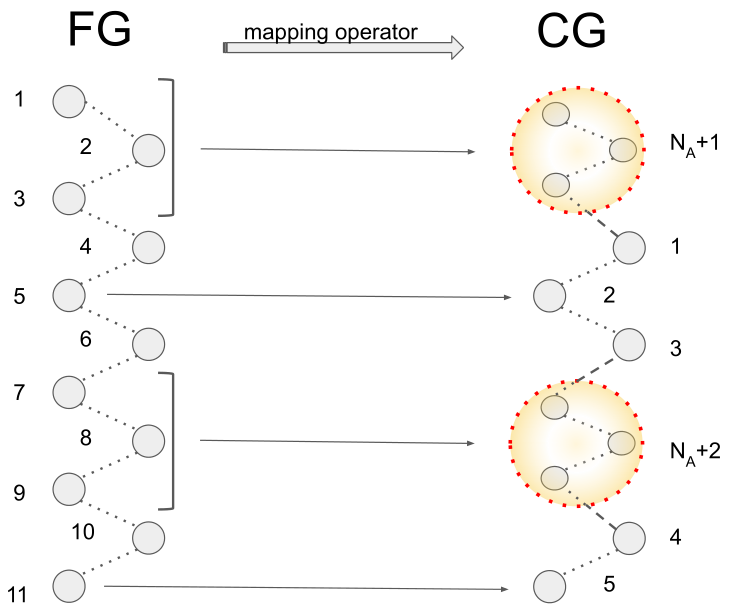
\includegraphics[width=\textwidth]{CGmapping}
    \caption{Sketch of the mapping of a molecule from the FG system to the general CG (hybrid) system where the labels of the ``particles'' for the two different resolutions are highlighted. In the picture, $\ncg=7$ and $\NA{}=5$ therefore, $S_1=\{4\},\,S_2=\{5\},\,\ldots,\,S_5=\{11\},\,S_6=\{1,\,2,\,3\},\,S_7=\{7,\,8,\,9\}$.}
    \label{Fig:sketch}
\end{figure}

\section{A particular class of mapping operator}
\label{Sec:Mapping}
The mapping operators are a collection of functions defined in the FG system that specify the physical meaning of CG variables, i.e. CG variables will be observables of the FG system. They can be defined as the functions
$$\Psi,\Phi\colon  \real^{6\nfg}  \to  \real^{6\ncg}$$ such that 
\begin{align*}
\Aphase{}  &\mapsto \Psi(\Aphase{}) \eqqcolon \Bphase{\bfR}(\Aphase{})=\cip{\bfR_1,\ldots,\bfR_{\ncg}}\,,\\
\Aphase{}  &\mapsto \Phi(\Aphase{}) \eqqcolon \Bphase{\bfP}(\Aphase{})=\cip{\bfP_1,\ldots,\bfP_{\ncg}}\,.
\end{align*}
We choose the mapping operator in the \emph{class of linear canonical coarse-graining operators} (see Ref.~\cite{DiPasquale2019}) With this choice, we define the mapping operator that select the the centre of mass of a CG particle as a positional coordinate, and the relevant conjugate momentum, which is simply the sum of momenta of all ``atoms'' within the bead:
\begin{align}
	\bfR_{I}=\Psi_{I} (\Aphase{}) & = \frac{1}{M_I}\sum_{k\in S_I} m_k\bfr_k \,, \label{Eq:constr1} \\
    \bfP_{I}=\Phi_{I} (\Aphase{}) & = \sum_{k\in S_I}{\bfp_k}\,. \label{Eq:constr2}
\end{align}
Here $ M_I=\sum_{k\in S_I}m_k $ where $ I = 1,\dots,\ncg $. Naturally there are other ways to choose the mapping operator that can better characterize the behavior of the beads. This choice is a linear canonical transformation, and has the convenient feature that it is local: each transformed degree of freedom depends only on a small number of FG variables, all of which are close to one another in space.

\section{Separability and effective interactions}
Generally the Hamiltonian of a molecular system consists of a kinetic part and a potential part consisting of a sum of 2, 3, and 4-body interactions. In the case of a hybrid system we can decompose the potential part as a sum of
%
\begin{labeling}{$\pot^{AA}(\Aphase{})$}
\item[$\pot^{AA}(\Aphase{})$] interaction potentials between the particles in the CG system that are simply ``atoms'';
\item[$\pot^{BB}(\Aphase{})$] interactions between ``atoms'' that are grouped into beads in the CG system;
\item[$\pot^{AB}(\Aphase{})$] interactions involving both ``atoms'' which are part of beads and ``atoms'' which are not coarse-grained.
\end{labeling}
%
So we can write the potential part as
\begin{equation}\label{Eq:int}
	\pot(\Aphase{}) = \pot^{AA}(\Aphase{}) + \pot^{AB}(\Aphase{}) + \pot^{BB}(\Aphase{})\,.
\end{equation}

To write explicitly for a hybrid system eq.~(\ref{Eq:ZwanGLE}) we begin to write explicitly the term relating to the entropic contribution to the Helmholtz free energy,  eq.~(\ref{Eq:Entropy(FreeE)}). Considering a separable Hamiltonian and a CG mapping of the form chosen in eq.~(\ref{Eq:constr1}) and eq.~(\ref{Eq:constr2}), the integral given by the \emph{structure function} eq.~(\ref{eq:structurefunc}) can be factorised into contributions arising from the momenta of CG particles and their positions, which results in the decomposition
\begin{align*}
  \entropy(\Bphase{}) &= -\frac{1}{\beta}\ln{}\biggl(
  \int{\frac{1}{\mathcal{Z}} \exp{{-\beta \Ham(\Aphase{})}}} 
    \dirac{\Psi\cip{\Aphase{}}-\Bphase{\bfR}}\dirac{\Phi\cip{\Aphase{}}-\Bphase{\bfP}}\diff\Aphase{}
    \biggr) = \\ 
    &= \entropy_{\bfP}(\Bphase{\bfP})+ \entropy_{\bfR}(\Bphase{\bfR}).   \nonumber 
\end{align*}
These terms were determined by Di Pasquale \textit{et al.} in their work \cite{DiPasquale2019} and are given by 
\begin{align}
 \label{Eq:MomB}
 \entropy_{\bfP}(\Bphase{\bfP}) & = {\sum_{I=1}^{\ncg}{\frac{|\bfP_{I}|^2}{2M_{I}}}} + const\,;\\
 \label{Eq:EntrInt}
 \entropy_{\bfR}(\Bphase{\bfR}) &= \pot^{AA}\Big(\{\bfR_I\}_{I=1}^{\NA{}}\Big) + \Veff(\Bphase{\bfR})\,;
\end{align}
where the first term is the kinetic energy of the CG particles, while the second one is the potential energy of the CG particles, with $\Veff$ being given by
\begin{equation*}
 \Veff = - \frac{1}{\beta} \ln{}  \cip{\int{\diff\Aphase{\bfr}' \frac{1}{\mathcal{\mathcal{Z}_{\bfR}}}
    \exp{\big[{{-\beta \big(\pot^{AB}(\{\bfR_I\}_{I=1}^{\NA{}},\bfr') +\pot^{BB}(\bfr') \big)}\big]}}}
    \prod_{J=\NA{}+1}^{\NB{}}\dirac{\Psi_{J}(\bfr')-\bfR_{J}}}
\end{equation*}
This term can be interpreted as an \emph{effective potential} due to the property that if $I$ satisfies $S_I=\{k\}$, then
%
\begin{equation}\label{Eq:ForceAt}
	-\pard{\Veff}{\bfR_I} = \aver{-\pard{\pot^{AB}}{\bfr_k}}_{\Bphase{}} =  \aver{\bfF_k}_{\Bphase{}}
\end{equation}
%
where $\bfF_k$ is the force acting on atom $k$ in FG system, which corresponds to particle $I$ in the CG system.
A similar result can be obtained for beads:
%
\begin{align}\label{Eq:VeffB}
	-\pard{\Veff}{\bfR_{J}} = \aver{-\sum_{k\in S_J}\frac{M_J}{m_k s_J}\pard{}{\bfr_k}\cip{\pot^{AB}+\pot^{BB}}}_{\Bphase{}} 
	= \aver{\Phi_J(\bfF)}_{\Bphase{}}
\end{align}
%
where $\Phi_J(\bfF)$ is the sum of the forces acting on the ``atoms'' within bead $J$. We stress that this definition of $\Veff$ is still formal and, in general, cannot be calculated analytically as it depends on all the coarse-grained variables. In order to make this definition implementable in numerical simulations, further approximations and assumptions will be necessary.

\section{Projected dynamics}
\label{sec:projcoor}
We now explicitly write the projected dynamics using the definitions of $\Phi,\Psi$ given in Sec.~\ref{Sec:Mapping}. We report below the results obtained by Di Pasquale et al. in their work \cite{DiPasquale2019}. The dynamics of $\Bphase{}(\Aphase{})$, that is, the dynamics for the position and momenta of a particle $\{\bfR_{J},\bfP_{J}\}$ in the CG system is given by
%
\begin{align*}
	\Lio\bfR_{J} & = \sum_{k\in S_J}{\frac{\bfp_k}{m_k}\pard{\Psi_J(\Aphase{\bfr})}{\bfr_k}}  = \sum_{k\in S_J}{\frac{\bfp_k}{m_k}\frac{m_k}{M_J}}  = \frac{\bfP_J }{M_{J}}  \\
	\Lio\bfP_{J} & = -\sum_{k\in S_J}{\pard{\pot(\Aphase{\bfr})}{\bfr_k}}\pard{\Phi_J(\Aphase{\bfp})}{\bfp_k}  = -\sum_{k\in S_J}{\pard{\pot(\Aphase{\bfr})}{\bfr_k}}
\end{align*}
%
To simplify the notation we introduce the operators $\Lio_\pproj \equiv \pproj_{\Bphase{}}\Lio$ and $\Lio_{\qproj} \equiv \qproj_{\Bphase{}}\Lio$, respectively the operators of projection and the orthogonal projection of the Liouvillian.

\noindent
The projected dynamics for the CG positions is given by 
\begin{equation*}
    \Lio_\pproj\bfR_{J} = \frac{\bfP_J}{M_J} \quad\text{and}\quad \Lio_\qproj\bfR_{J} = 0\,. 
\end{equation*}
While for the CG momenta, the projected dynamics are given by
%
\begin{equation*}
  \begin{aligned}
    \Lio_\pproj\bfP_{I} & = -\pard{\pot^{AA}}{\bfR_I} - \pard{\Veff}{\bfR_{I}}	&\quad&\text{for }I=1,\ldots,\NA{},\text{ with }S_I=\{k\},&\\
    \Lio_\pproj\bfP_{J} & = - \pard{\Veff}{\bfR_{J}}	 &\quad&\text{for }I=\NA{}+1,\ldots,\ncg,&
  \end{aligned}
\end{equation*}
% 
and therefore the orthogonal projections are
%
\begin{align*}
  \Lio_\qproj\bfP_{I} &= -\pard{\pot^{AB}}{\bfr_k}  + \pard{\Veff}{\bfR_I} &  & \text{for }I=1,\dots,\NA{},\text{ with }S_I=\{k\}\,,\\
  \Lio_\qproj\bfP_{J} &= -\sum_{k\in S_J}{\pard{}{\bfr_k}\cip{\pot^{AB}+\pot^{BB}} } + \pard{\Veff}{\bfR_J} &  & \text{for }I=N^A+1,\dots,\ncg\,.
\end{align*}
% 
These functions are often referred to as \emph{fluctuating forces}. So we can rewrite the eq.~(\ref{Eq:RAndomForce}) for a generic $t$ as 
\begin{equation}
\label{Eq:StocFor}
 \fprojbf_{I}(t,\cdot) = \exp{t\Lio_\qproj}\Lio_\qproj\bfP_I(\cdot) \quad \text{for } I=1,\dots,\ncg.
\end{equation}


\section{Final system of equations}
Finally, we can rewrite the GLE (\ref{Eq:ZwanGLE}) as 
\begin{align}
 \nonumber
 \pard{\bfR_{K}}{t} &= \frac{\bfP_{K}}{M_{K}} \\
 \nonumber 
 \pard{\bfP_{K}}{t} &= -\omega_{\NA{} K} \pard{\pot^{AA}}{\bfR_{K}} - \pard{\Veff}{\bfR_{K}} 
 - \sum_{J=1}^{\ncg}\,\int_{0}^{t}\,\fricmat_{KJ}(t-s,s)\,M_J^{-1}\,\bfP_J(t-s) \,\diff s \\
 &+ \beta^{-1} \sum_{J=1}^{\ncg} \,\int_{0}^{t} \pard{\fricmat_{KJ}(s)}{\bfP_{J}} \,\diff s + \fprojbf_{K}(t)
 \label{Eq:DevB} 
\end{align}
%
where $\omega_{N^AK}$ is equal to zero whenever the difference between the first and second subscript is negative and one otherwise.


\section{Orthogonal Dynamics}
\label{Sec:OD}
Following the work of Di Pasquale \textit{et al.} we can determine the orthogonal dynamics by means of the constrained dynamics \cite{DiPasquale2019}. Where 
the constraints are given by the mapping operators (see Sec.~\ref{Sec:Mapping}), and can be written as:
%
\begin{align*}
	\Psi_I(\bfr) - \bfR_I & = 0\,, \\
	\Phi_I(\bfp) - \bfP_I & = 0\,.
\end{align*}
%
The equation of motion for the constrained dynamics are given by:
%
\begin{align}
	\nonumber
	\totd{\bfr_k}{t} &= \frac{\bfp_k}{m_{k}} - \frac{\bfP_I}{M_I} \\
	\label{Eq:orth}
	\totd{\bfp_k}{t} &= - \pard{U(\Aphase{\bfr})}{\bfr_k} + \frac{m_k}{M_I}\sum_{i\in S_I}\pard{U(\Aphase{\bfr})}{\bfr_i}%\bfF_I\label{Eq:orth} 
\end{align}
%
where $I$ is the index such that $k\in S_I$.

\chapter{Markovian approximation}
\label{Sec:MarkovApprox}

The terms involving the friction matrix turn out to be the most difficult to compute in a real calculation because of the memory effect. 
The problems to be faced in order to simplify the formulation of the eq.~(\ref{Eq:ZwanGLE}) are given by:
\begin{itemize}
\item[-] the calculation of the friction matrix $\bffricmat(t)$ eq.~(\ref{Eq:FRICmatrixRF}), which depends on the orthogonal dynamics, i.e., on all the fast degrees of freedom that one wants to coarse-grain away (see eq.~(\ref{Eq:RAndomForce}));   
\item[-] the integrals that include the friction matrix, which must be computed at each time step (see the RHS of the eq.~(\ref{Eq:ZwanGLE})).
\end{itemize}
In the literature there are different ways to consider the friction matrix \cite{Chorin2000,Kauzlaric2011} and how to include memory effects in CG simulations \cite{Izvekov2017,Jung2017,Li2015,Yuanran2018}.

In many cases, it has been shown that $\bffricmat(\Bphase{},t)$ exhibits a fast exponential decay in $t$ and uniformly on the phase-space, so that the integrals involving the memory kernel may be approximated using an asymptotic expansion of integrals (see Ref.~\cite{bernardini1993Metodi,bleisteinAsExpInt,DiPasquale2019}). If the exponential characteristic time is much shorter than the characteristic time scale of the CG model, then the latter can be regarded as memoryless. This is the most common approximation used, which corresponds to assuming that the CG models satisfy the property that allows to predict the future with only the present information. This property is the so-called ``Markov property''.
The validity of the Markovian assumption requires a clear separation of the time scales of the system under examination \cite{DiPasquale2019,Hijon2010,Hijon2006}.
In particular, in the studied system the assumption is valid only if the time scale of variation of the CG variables is much larger than the time scale of decay of the memory matrix $\bffricmat(t)$ (i.e., the friction matrix), which is linked to the time scale of the autocorrelation of the fluctuating forces $\fprojbf_{\Bphase{}}(t,\cdot)$, defined in eq.~(\ref{Eq:RAndomForce}).

Therefore, to simplify and numerically implement the eq.~(\ref{Eq:ZwanGLE}), we assume that the model under examination satisfies the Markov property and that the friction matrix can be approximated as
\begin{equation*}
  \bffricmat(\Bphase{},t) = \exp{-\lambda t}f(\Bphase{},t)
\end{equation*}
where $f$ is a slowly-varying continuous function in the interval of integration and the parameter $\lambda$ is the inverse of a mesoscopic time-scale that is larger than the microscopic characteristic time but much smaller than the macroscopic one~\cite{Berne:DynamicLightScatt,Hijon2010}. 
We can rewrite the first integral of the second equation of the system~(\ref{Eq:DevB}) as
\begin{multline}
\label{Eq:TermIntMARapp}
  \int_0^t\, \bffricmat(\Bphase{}(t-s),s) \cdot(M^{-1}\bfP) \,\diff s ={}\\
   = \int_0^t\, \exp{-\lambda s}f(\Bphase{}(t-s),s) \cdot(M^{-1}\bfP) \,\diff s = \frac{1}{\lambda}\, f(\Bphase{}(t),0) \cdot (M^{-1}\bfP) 
   + O(\lambda^{-2}) ={}\\ 
   = \frac{1}{\lambda}\, \bffricmat(\Bphase{}(t),0) \cdot (M^{-1}\bfP) + O(\lambda^{-2}) 
   =  \widetilde{\bffricmat}(\Bphase{}) \cdot (M^{-1}\bfP) + O(\lambda^{-2}).
\end{multline}
which has been derived by integrating by parts and noting that the absolute difference between the original integral and the border term is asymptotically limited by the integral term obtained by integrating by parts, which is of the order of $\lambda^{-2}$ and hence, since $1 / \lambda$ is much smaller than the macroscopic timescale, can be neglected. This can be verified by applying the Watson lemma (see pp.199-203 Ref.~\cite{bernardini1993Metodi}). In eq.~(\ref{Eq:TermIntMARapp}) $\widetilde{\bffricmat}$ is the time-independent friction matrix defined as	
\begin{equation}\label{Eq:MarDeltaFric}
  \widetilde{\bffricmat}(\Bphase{}) \coloneqq \frac{1}{\lambda}\,\bffricmat(\Bphase{}(t),0)
  = \frac{1}{\lambda}\, \beta\aver{\fprojbf_{\Bphase{}}(0,\cdot)\otimes
    \fprojbf_{\Bphase{}}(0,\cdot)}_{\Bphase{}}\,.
\end{equation}
Since $\widetilde{\bffricmat}$ does not depend on the momenta (see eq.~(\ref{Eq:StocFor})), its derivative with respect to ${\bf P}$ is zero, and therefore the second integral in the RHS of the second equation of the system~(\ref{Eq:DevB}) vanishes.

\noindent
Under these assumptions, the second equation of the system (\ref{Eq:DevB}) becomes
\begin{equation}	
 \label{Eq:MarkovApprox}
  \pard{\bfP_{K}}{t} = -\omega_{\NA{}K} \, \pard{\pot^{AA}}{\bfr_{K}} 
                       -\pard{\Veff}{\bfR_{K}}
                       - \sum_{J=1}^{\ncg}\, \widetilde{\fricmat}_{KJ} \, \frac{\bfP_{J}}{M_{J}} 
                       + \fprojbf_{K}(t)\,,         
\end{equation}
where the time-independent friction matrix is a symmetric matrix, \textit{i.e.} $\widetilde{\fricmat}_{KJ}=\widetilde{\fricmat}_{JK}$. This is easy to verify, since by making the terms explicit in the definition (\ref{Eq:MarDeltaFric}) we obtain
\begin{multline}
\label{Eq:convFlucF}
  \aver{\fprojbf_K(0,\cdot) \otimes \fprojbf_J(0,\cdot)}_{\Bphase{}} = \aver{\Lio_\qproj\bfP_K \otimes \Lio_\qproj\bfP_J}_{\Bphase{}} ={}\\
  = \aver{ \cip{ \pard{\Veff}{\bfR_{K}} - \sum_{i\in S_K} \pard{U}{\bfr_{i}} } 
  \cip{ \pard{\Veff}{\bfR_{J}} - \sum_{j\in S_J} \pard{U}{\bfr_{j}} }}_{\Bphase{}}\,.
\end{multline}
In the past, the validity of the Markovian approximation has been questioned~\cite{CommentCubero,Cubero2005,Hijon2006,ResponseCommentHijon}. We will return to this point later when we discuss the numerical results. We want to stress here that we use the Markovian approximation only as a means of simplifying the calculation. As we said at the beginning of this section there are more refined methods to consider the friction matrix and to include memory effects in CG simulations, but in this work we will consider only the Markovian approximation, as our main goal is to show the differences in the results for the different terms composing the GLE and the comparison with the results reported in the work of Di Pasquale \textit{et al.}~\cite{DiPasquale2019}.


\chapter{Numerical Methods}
\label{Sec:NumMet}

\section{Langevin Dynamics Integrator: the BAOAB method}
In this thesis the Langevin Dynamics is integrated by using the BAOAB method, which was derived and analysed by B. Leimkuhler and C. Matthews \cite{LeimMatt:LAnDynInt}. 

The aim of their work is to compare Langevin dynamics integrators in term of their invariant distributions and demonstrate a superconvergence property of a certain method in the high friction limit (or in the null mass limit). They coded up the various methods considered and compared the accuracy of configurational sampling for different values of the friction parameter $\gamma$ and for a range of timesteps.

Their results show that the best method to sample the configurational Gibbs-Boltzmann distribution\footnote{This means that the calculation of averages of functions of phase space variables of a molecular N-body system modelled at constant temperature.} is the BAOAB method, which is an efficient and easy-to-implement scheme using a single force vector per timestep:
\begin{align*}
 p_{n+1/2} &= p_n-\frac{1}{2}\,\nabla U\left(x_n\right)\,dt\,; \\
 x_{n+1/2} &= x_n+\frac{1}{2}\,M^{-1}\,p_{n+1/2}\,dt\,; \\
 \widehat{p}_{n+1/2} &= c_1\,p_{n+1/2}+c_2\,M^{1/2}\,R_{n+1}\,; \\ 
 x_{n+1} &= x_{n+1/2}+\frac{1}{2}\,M^{-1}\,\widehat{p}_{n+1/2}\,dt\,; \\
 p_{n+1} &= \widehat{p}_{n+1/2}-\frac{1}{2}\,\nabla U\left(x_{n+1}\right)\,dt\,. \\
\end{align*}
Here, $R_i$ is an N-vector of normal random numbers with mean $0$ and variance $1$, $M$ is the diagonal mass matrix, $dt$ is the timestep, 
$c_1=e^{-\widetilde{\gamma}\,dt}$ and $c_2=\sqrt{\left(1-c_1^2\right)/\beta}$ are evaluated for a given friction parameter $\widetilde{\gamma}=\gamma\,M^{-1}$ and for a given temperature parameter $\beta=(K_BT)^{-1}$, where $K_B$ is the Boltzmann's constant.

\subsection{Some more details about the work of B. Leimkuhler and C. Matthews}
The methods that are considered are splitting integrators that decompose the stochastic vector field which drives the Langevin Dynamics into simpler vector fields which can be solved exactly. Nevertheless, the composition method that results cannot be directly related to a stochastic differential equation, but nonetheless the invariant measure associated to the numerical method can be derived, using the Baker-Campbell-Hausdorff (BCH) expansion \cite{bernardini1993Metodi,evans2008}, as an asymptotic series in two parameters: the stepsize and the coefficient $\gamma^{-1}$. 

The authors stress that their approach focuses on the truncation error of the invariant distribution, so that the greatest benefit would be seen only when the statistical error is well controlled. Furthermore, they observe that the least biased scheme from the point of view of the error introduced in configurational sampling is also as efficient as the alternatives and the most robust with respect the variation of parameters (stepsize and $\gamma^{-1}$).


\section{Constrained Langevin Dynamics Integrator: the geodesic BAOAB method}
We now present an integrator for constrained stochastic dynamics such as Langevin dynamics for holonomic constraints, developed by by B. Leimkuhler and C. Matthews \cite{Leimkuhler2016}. 

Their approach to Langevin dynamics in the presence of constraints is based on the decomposition of the system into three components representing a geodesic flow, a constrained impulse and a constrained diffusion. In fact, their idea is to divide the problem of the constrained MD into a collection of separate constrained problems and to solve or approximate each constrained flow. 

The Hamiltonian dynamics is split into potential and kinetic terms, and Lagrange multipliers are introduced to maintain the constraints. The solution of the part defined by the potential energy can be obtained easily, while the solution of the kinetic part is a geodesic curve (an unforced motion on the constraint surface) and requires solving a non-linear system of ordinary differential equations (ODE). In practice, the geodesic is approximated using a series of SHAKE/RATTLE steps \cite{ANDERSEN1983,RYCKAERT1977} that preserve the constraint manifold and respect the cotangency conditions, \textit{i.e.}, the constraints on the momenta. 

The resulting procedure is a ``geodesic integrator'' that solves the two parts separately and then recomposes the flows.
The algorithm thus represents a geodesic version of their BAOAB integrator presented in the previous section.


\part{Numerical Experiments}
\label{Sec:NumExp}

\chapter{The system under study}
In Chapter \ref{Sec:CanMapp&CG}, we derived the general structure of the equations of motion for generic CG (hybrid) system. Here, we numerically investigate the effects of some of the choices and assumptions made when the FG system is coarse-grained in the canonical ensemble. To do this, we have extended the numerical implementation and the analysis made by Di Pasquale \textit{et al.}~\cite{DiPasquale2019}. 

Di Pasquale \textit{et al.}~developed an open-source parallel code, written in Julia v0.6.2 \cite{thomas_hudson_2018_1226590}, to solve the full, constrained and coarse-grained dynamics in the microcanonical (NVE) ensemble for a simple one-dimensional system. To extend the code to the canonical (NVT) ensemble we introduced the integrators described in the Chapter \ref{Sec:NumMet}, after updating the code to the latest version of Julia, v1.2.0.

The studied system is a linear periodic chain made of $\nfg$ atoms of two different species, which differ in mass and bond stiffness. The atoms are arranged in a repeating pattern, and the coarse-grained model is obtained by combining the single repeated units into beads, see fig.~\ref{Fig:sketchRepPatt}. Therefore, we will not consider a hybrid system, and the number of beads, $\ncg$, will be equal to the number of times the pattern is repeated in the chain. The CG variables are given by the center of mass of each bead and by the corresponding momenta (see section \ref{Sec:Mapping}).
\begin{figure}[htb]
 \centering
 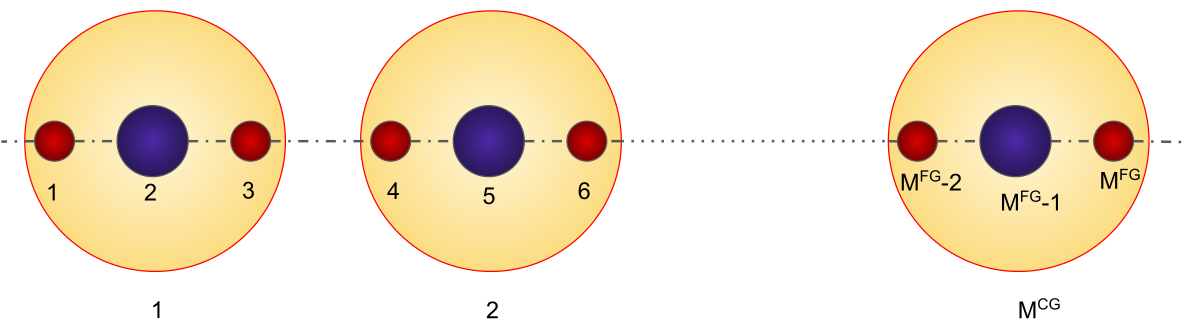
\includegraphics[width=0.95\textwidth]{chain}
 \caption{Sketch of the one-dimensional chain composed by $\nfg$ atoms of two different species. The two species are indicated as red and blue particles, differing in mass and bond stiffness. Small red spheres represent atoms of mass $m$ and big blue spheres represent atoms of mass $M$. Beads are indicated as yellow spheres that surround three atoms each.}
 \label{Fig:sketchRepPatt}
\end{figure}

This system is the same studied by Di Pasquale \textit{et al.}, who have studied such a simple system to understand and quantify the accuracy of various modelling assumptions. We made this choice to directly compare the results obtained here with those of Ref.~\cite{DiPasquale2019}, and to compare the results obtained in the two ensemble.

\section{Test cases considered}
\label{Sec:TestCasesConsid}

The studied test cases are composed of atoms with two different masses, set to $m=1$ and $M=10$.
The repeating pattern  consists of three atoms in two different configurations: two atoms of mass $m$ and a single atom of mass $M$ ($m-M-m$) or vice versa ($M-m-M$). The number of beads is set to $\ncg=10$, so that the number of atoms is also fixed, $\nfg=3\,\ncg=30$.
The bond stiffness between the two different species of atoms is described by means of an inter-atomic potential, which is a simple 12-6 Lennard-Jones potential. In the following, all parameters, such as temperature and time step, are expressed in terms of dimensionless units, \textit{i.e.} the so-called Lennard-Jones reduced units.These dimensionless units are obtained by using $\epsilon$, $\sigma$, $\sigma(m/\epsilon)^{1/2}$ and $\epsilon/K_B$ as fundamental units of energy, length, time and temperature, respectively (\textit{e.g.}~see Tuckerman pp.125-127 Ref.~\cite{tuckerman2010}). 
The canonical (NVT) ensemble was implemented by introducing a thermal bath with a friction parameter $\gamma=1$, and setting the temperature so that $\beta=(K_B\,T)^{-1}=1.096$.
Following the work of Di Pasquale \textit{et al.}, we assume periodic boundary conditions and nearest neighbour interactions. 
The inter-atomic potential for a generic system $X$ is given by 
\begin{equation}
 \begin{split}
  	\pot^X_{i,i+1}(r) &= 4\,\epsilon_{i,i+1} \sqp{\cip{\frac{\sigma_{i,i+1}}{r}}^{12} - \cip{\frac{\sigma_{i,i+1}}{r}}^6} ={}\\
	&= \epsilon_{i,i+1} \sqp{\cip{\frac{r^*_{i,i+1}}{r}}^{12} - 2\cip{\frac{r^*_{i,i+1}}{r}}^6} \,.
 \end{split}
\end{equation} 
Here, we choose $\sigma_{i,i+1}=2^{-1/6}$ so that the minimum value of the potential is obtained for $r^*_{i,i+1}=1$, while the well-depth will be varied to analyse the effect of the stiffness of the interactions: $\epsilon_{i,i+1}\in\bp{0.1,1,100}$. The interaction between two different species of atoms is set by the so-called Lorentz-Berthelot mixing rule. The parameters $\epsilon_{i,i+1}$ are thus given by
\begin{equation}
  \epsilon_{i,i+1} = \begin{cases}
    \sqrt{\epsilon_\alpha\epsilon_\beta} & i = 1,\, 2,\, 4,\, 5,\, \dots,\, \nfg-2,\, \nfg-1; \\
    \epsilon_\alpha\;\;(\mbox{or}\,\,\epsilon_\beta) & i = 3,\, 6,\, \dots,\, \nfg;
  \end{cases}
\end{equation}
where $\epsilon_\alpha$ and $\epsilon_\beta$ are two different values for the parameter $\epsilon$ taken from the set $\bp{0.1,1,100}$.
The Hamiltonian is given by
\begin{equation}
 \begin{split}
  	\Ham^X(\bfr,\bfp) &= \frac12 \, \bfp^T\,(M^X)^{-1}\,\bfp\,+\sum_{i=1}^{\nfg-1}\pot^X_{i,i+1}\cip{\bfr_{i+1}-\bfr_i}\,+ \\
	&+ \pot^X_{\nfg,1}\cip{\bfr_1-\bfr_\nfg+r^*\nfg},
 \end{split}
 \label{eq:1DHamiltonian}
\end{equation}
where $M^X$ is the mass matrix, $\bfr$ and $\bfp$ are respectively the positions and momenta of the atoms in the system $X$ considered. 
The final term takes into account that periodic boundary conditions are in place, \textit{i.e.}, that the two ends of the linear chain behave as if they were connected to each other.

We considered four test cases denoted as $A$, $B$, $C$, $D$:
\begin{itemize}
 \item the pairs $A$ and $B$, and $C$ and $D$ have the same repeating pattern  ($m-M-m$ and $M-m-M$, respectively) but different interactions among the atoms;
 \item the pairs $A$ and $C$, and $B$ and $D$ have the same intra-beads interactions (\textit{i.e.} interactions among atoms belonging to the same bead) and the same inter-beads interactions (\textit{i.e.} interactions among atoms in different beads). Of course they have a different repeating pattern and consequently different masses.
\end{itemize}
A summary of the four cases, with all the parameter values used, is given in the table \ref{Tab:Cases}.
\begin{table}[htb]
 \centering
 \begin{tabular}{c c c c c c} 
  \toprule[1.1pt]
   &  & \multicolumn{4}{c}{Interactions ($\epsilon_{i,i+1}$)} \\
  \cmidrule(l){3-6}
  System & Bead structure & $m-m$ & $M-M$ & $m-M$ & Inter-bead \\
  \midrule
  $A$ & $m-M-m$ & $1$ & $100$ & $10$ & $1$ \\ 
  $B$ & $m-M-m$ & $10$ & $0.1$ & $1$  & $10$ \\  
  $C$ & $M-m-M$ & $100$ & $1$ & $10$ & $1$ \\
  $D$ & $M-m-M$ & $0.1$ & $10$ & $1$ & $10$ \\
  \bottomrule[1.1pt]
 \end{tabular}
 \caption{Summary of parameters in the 4 configurations considered. Intra-beads interactions are always between atoms of different masses ($m-M$), while inter-bead interactions are between atoms of the same mass ($m-m$ or $M-M$ depending on the case under consideration).}
 \label{Tab:Cases}
\end{table}

The dynamics were implemented using the integrators described in the Chapter \ref{Sec:NumMet}. The time step chosen was $\Delta t=10^{-3}$, which is smaller than the shortest timescale in the system: $\Delta t \leq min\;\sqrt{M/\pot^{''}_{i,i+1}(1)}\approx 5.89 \times 10^{-3}$, see \cite{DiPasquale2019}.   
Below, we will show the results and analysis of the simulations of different dynamics:
\begin{labeling}{(MMZD)}
\item[(FGD)] the \emph{Fine-Grained Dynamics} when solving eq.~(\ref{Eq:MotionEq}) with the Hamiltonian defined in eq.~(\ref{eq:1DHamiltonian}):
 \[
 \totd{\Aphase{}(t)}{t} = \bp{\Aphase{},\Ham^X} = iL\,\Aphase{}\,;
 \]
\item[(OD)] the \emph{Orthogonal Dynamics} when solving the system of eq.~(\ref{Eq:orth}):
 \[
  \totd{\bfr_k}{t} = \frac{\bfp_k}{m_{k}}- \frac{\bfP_I}{M_I} \,;\qquad
  \totd{\bfp_k}{t} = - \pard{\pot^X(\Aphase{\bfr})}{\bfr_k} + \frac{m_k}{M_I}\sum_{i\in S_I}\pard{\pot^X(\Aphase{\bfr})}{\bfr_i}\,; 
 \]
\item[(CGD)] the \emph{Coarse-Grained Dynamics} when solving eq.~(\ref{Eq:MarkovApprox}) for a fully coarse-grained system, neglecting the dissipative and fluctuating terms:
 \[
 \pard{\bfR_{K}}{t} = \frac{\bfP_{K}}{M_{K}}\,; \qquad
 \pard{\bfP_{K}}{t} = -\pard{\Veff}{\bfR_{K}}\,;  
 \]
\item[(MMZD)] the \emph{Markovian Mori-Zwanzig Dynamics} when solving eq.~(\ref{Eq:MarkovApprox}) for a fully coarse-grained system, with the memory and fluctuating terms replaced by a position-dependent Langevin dynamics, \textit{i.e.}, memory and fluctuating terms that depend on the inter-particle distance.
\end{labeling}
As we said, in order to numerically integrate the FGD and OD we have used respectively the BAOAB and geodesic-BAOAB integrators (see Chapter \ref{Sec:NumMet}). By contrast, to numerically integrate the MMZD we have used a version of the BAOAB integrator adapted to the case of non-constant diffusion, developed by Di Pasquale \textit{et al.}~\cite{DiPasquale2019}. 

\section{Sampling Algorithm}

The developed code allows a relatively simple recalibration of the test system through Julia ``types'', which are initialized by the user to fix all the parameters of the simulation, including the repeating pattern of the beads, the number of beads, the mass and stiffness of the inter-atomic potentials.
Here, we give an idea of the sampling implemented in the code to compute an approximation of the effective potential, given in eq.~(\ref{Eq:EntrInt}), and the friction matrix, as given in eq.~(\ref{Eq:FRICmatrixRF}). The idea is to sample using the OD.

First, the initial conditions for the simulation are fixed, so that the momenta are distributed according to the Maxwell-Boltzmann distribution and the positions lie in a neighbourhood of the equilibrium positions, determined by the equilibrium distance of the inter-atomic potential.
Then the trajectory of the FGD is computed and samples of the positions and momenta are stored. These samples are used to determine the CG positions and momenta, and are used as initial condition for computing the trajectories of the OD. Along these trajectories, time averages of the first and second moment of the effective force between beads are stored. The first moment gives the value of the mean force acting between adjacent beads given the position of the center of mass, while the second moment is used to compute the friction matrix. Since the sampling steps of the OD can run at the same time without having to communicate between the processes, these procedures can be run in parallel. 
Finally, by integrating the mean force with respect to the distance $R$ between the beads, the effective potential $\Veff$ is obtained.

This method is very similar to the force-matching method \cite{Ercolessi1994,Izvekov2004}, the difference being that here we derive directly the effective potential from the sampling performed during the OD simulations.
Below, for further clarification of what we said, we report the algorithm published in the work of Di Pasquale \textit{et al.}~and implemented in the code:
\begin{algorithm} [H]
\caption{Sampling Algorithm \cite{DiPasquale2019}}
\begin{algorithmic}[1]
  \Procedure{Constrained Sample}{Configuration of atomistic system, target$_1$, target$_2$}
  \State Generate initial condition for fine-grained system
   \While{$\#$ of samples $<$ target$_1$}
   \State Run FGD to generate initial condition for constrained dynamics (OD)
   \While{length of constrained dynamics trajectory $<$ target$_2$}
   \State Advance the timestep using the integrator for the constrained dynamics
   \State Update statistical estimators
   \EndWhile
   \EndWhile
\EndProcedure
\end{algorithmic}
\end{algorithm}

\chapter{Simulation results}
\section{Data-driven approximation of the effective potential}
\label{Sec:EP}
In order to improve the time required to sample the mean force, and thus determine the effective potential, we use the translational symmetry of this simple system, the fact that the beads are identical and the assumption that the effective potential can be approximated as a sum of two-body interactions based on the distance to the nearest-neighbour beads only.
We thus compute the interactions between any combination of beads and assume that the interactions computed are valid for any equivalent pair in the system. In this way we reduce the dimensionality of the space to be sampled from the total number of coarse-grained variables to simply one, \textit{i.e.}, the inter-bead distance, which simplifies the exploration of the entire constrained phase space, as well as the representation and interpolation of the effective potential in the parameter space.

The validity of these assumptions in this simple system considered was verified by Di Pasquale \textit{et al.}~\cite{DiPasquale2019}. Naturally, in a more realistic system these assumptions could cause a significant deterioration in the accuracy and effectiveness of a systematic MZ projection approach.

In fig.~\ref{Fig:meanForce},
%
\begin{figure}[!htb]
 \centering
 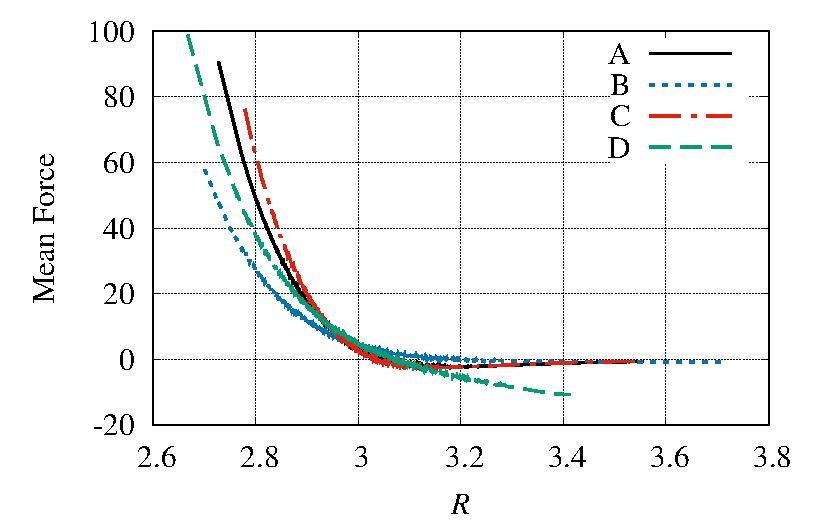
\includegraphics[width=\textwidth]{sABCD_2000_MF}
 \caption{Plot of the mean force for the four systems considered (see table \ref{Tab:Cases}) \textit{versus} the inter-bead distance $R$: system A (black solid line), system B (dotted blue line), system C (red dashed-dotted line) and system D (dashed green line). 
 %\lr{perché la curva di D non tende a 0 per $R \to \infty$?}
}
 \label{Fig:meanForce}
\end{figure}
%
we show the results of the computation of the mean force for the four different systems described in the table \ref{Tab:Cases}. In each case, the trend is rather similar and we observe that the equilibrium bond length lies close to $R=3.0$. As expected, these results are consistent with the ones obtained by Di Pasquale \textit{et al.}~in the microcanonical (NVE) ensemble.

In fig.~\ref{Fig:FF},
%
\begin{figure}[!htb]
 \centering
 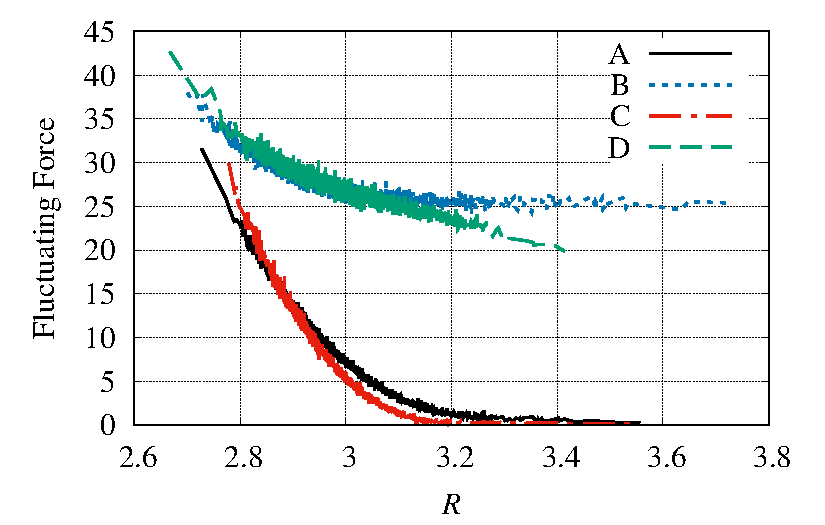
\includegraphics[width=\textwidth]{sABCD_2000_FF}
 \caption{Plot of the fluctuating part of the force for the four systems considered (see table \ref{Tab:Cases}) \textit{versus} the inter-bead distance $R$: system A (black solid line), system B (dotted blue line), system C (red dashed-dotted line) and system D (dashed green line). 
%\lr{Perché le fluttuazioni di B e D non tendono a 0 per $R \to \infty$?}
}
 \label{Fig:FF}
\end{figure}
%
we report the results for the fluctuating part of the force. First of all we note that the coupling to the thermal bath considered here yields curves with a much smaller noised compared to the work of  Di Pasquale \textit{et al.}~\cite{DiPasquale2019}. Interestingly, unlike the mean force, the two systems with the same stiffness (see table \ref{Tab:Cases}) follow a similar trend. In particular the two systems with the smallest stiffness, systems B and D, have noisier and larger fluctuations than the other two.  
Furthermore, the figure shows how these simple systems have a dependence of fluctuations on the inter-bead distance $R$, and consequently shows how a simple Langevin dynamics, with dissipation and white noise fluctuations having a magnitude independent of the state of the system,  might not be an adequate approximation.
%\lr{questo è uno spunto interessante... puoi espandere secondo te? Mettere delle referenze?}

The plots of the mean force and the fluctuating force (fig.~\ref{Fig:meanForce} and fig.~\ref{Fig:FF}, respectively) show that the majority of the points lies within the $[2.8,3.2]$ region, whereas distances outside of this range are rarely accessed. We will clearly show later, when we will discuss the distribution of the inter-bead distances for the various dynamics (FGD, CGD and MMZD, Sec.~\ref{Sec:Observables}), that this is indeed due to a lower probability of sampling.

Finally in fig.~\ref{Fig:EP}, we show the effective potential, obtained by integration of the mean force (fig.~\ref{Fig:meanForce}) with respect to the inter-bead distance $R$.
\begin{figure}[!htb]
 \centering
 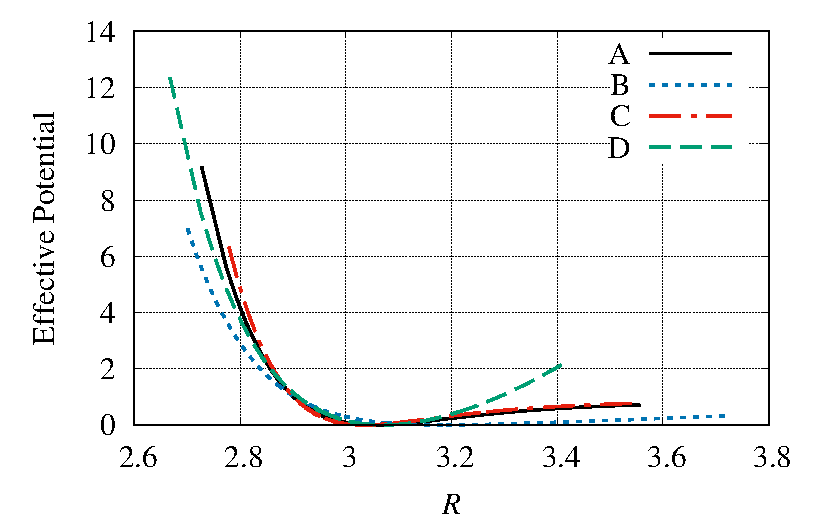
\includegraphics[width=\textwidth]{sABCD_2000_EP}
 \caption{Plot of the effective potential for the four systems considered (see table \ref{Tab:Cases}) \textit{versus} the inter-bead distance $R$: system A (black solid line), system B (dotted blue line), system C (red dashed-dotted line) and system D (dashed green line). 
 %\lr{anche qui bisogna sistemare i dati a grandi $R$}
}
 \label{Fig:EP}
\end{figure}
We observe that the effective potential has similar trends for the four systems, despite the big difference in the fluctuations of the force shown in fig.~\ref{Fig:FF}. Our results thus show that, even when the effective potential is easily and stably computed, there may be dissipative effects that are not visible in a deterministic effective potential. 

We note that the two pairs of systems $A$ and $C$ and $B$ and $D$ differ only in the mass of their constituents, meaning that all the structural observables, such as the effective force or the effective potential should be the same. While the $A$ and $C$ systems do display the same behaviour, with differences ascribable to numerical noise, the $B$ and $D$ systems are markedly different. This difference, which might be due to the poorer sampling caused by the large value of the inter-bead interaction, shows that the results obtained with these systems are most likely not completely reliable and hence we will focus on the $C$ system in the following sections. 

\section{Memory kernel approximation and numerical implementation}
Until now, we have not yet shown how to implement eq.~(\ref{Eq:MarkovApprox}) to determine MMZD, but only sketched the basic idea in Sec.~\ref{Sec:TestCasesConsid}. We said that the MMZD is determined by the Langevin-type eq.~(\ref{Eq:Lang1Dp}), where the potential is given by the effective potential and the memory and fluctuating terms depends on the inter-bead distance. 

For the sake of clarity, we report below the system of equations for a coarse-grained system in the Markovian approximation obtained in the Chap.~\ref{Sec:MarkovApprox}:
\begin{equation}
\label{Eq:MarkovApproxCompact}
\begin{cases}
 \partial_t\,\Bphase{\bfR} = M^{-1}\Bphase{\bfP} \,, & \\
 \partial_t\,\Bphase{\bfP} = -\partial_{\bfR}\Veff 
                             - \widetilde{\bffricmat}(\Bphase{})\cdot \cip{M^{-1}\Bphase{\bfP}}
                             + \fprojbf(t) \,. &  
\end{cases}
\end{equation}
The components of the time-independent friction matrix, \textit{i.e.}, eq.~(\ref{Eq:MarDeltaFric}) 
\[
  \widetilde{\bffricmat}(\Bphase{}) \coloneqq \frac{1}{\lambda}\,\bffricmat(\Bphase{},0) =  
  \frac{1}{\lambda}\, \beta\, \cexpval{ \fprojbf_{\Bphase{}}(0,\cdot) \otimes \fprojbf_{\Bphase{}}(0,\cdot) }{ \Bphase{} }\,,
\]
can be computed by means of the fluctuating force (fig.~\ref{Fig:FF}).
If we consider bead $I$, which interacts with bead $I-1$ and bead $I+1$, we can assume that the forces that act on it can be decomposed as the independent ``stress'' contributions $\sigma_{I+1,I}$ and $-\sigma_{I,I-1}$. Under these conditions we write the $\fricmat_{I,I}$ component of the time-independent friction matrix as
\begin{align*}
  \fricmat_{I,I}(\bfR) = \beta\,\cexpval{\fprojbf_I \otimes \fprojbf_I}{\bfR} &=
           \beta\,\cexpval{ (\sigma_{I+1,I}-\sigma_{I,I-1}) \otimes (\sigma_{I+1,I}-\sigma_{I,I-1}) }{\bfR} = \\
  &= \beta\,\cexpval{ \sigma_{I+1,I} \otimes \sigma_{I+1,I} }{\bfR} + \beta\,\cexpval{ \sigma_{I,I-1} \otimes \sigma_{I,I-1} }{\bfR} \,,
\end{align*}
where we consider the cross terms to be negligible, \textit{i.e.},
\[
 \cexpval{ \sigma_{I+1,I} \otimes \sigma_{I,I-1} }{\bfR}\approx 0 \quad\text{and}\quad \cexpval{ \sigma_{I,I-1} \otimes \sigma_{I+1,I}}{\bfR}\approx 0\,.
\]
In other words, we assume the fluctuating forces between adjacent beads are not correlated, since we have made the assumption that pair interactions are sufficient to describe the behaviour of the system.

\noindent
In the same way, we obtain
\begin{align*}
 \fricmat_{I,I+1}(\bfR) &= \beta\,\cexpval{\fprojbf_I \otimes \fprojbf_{I+1}}{\bfR} = \\
 &= \beta\,\cexpval{ (\sigma_{I+1,I}-\sigma_{I,I-1}) \otimes (\sigma_{I+2,I+1}-\sigma_{I+1,I}) }{\bfR} = \\
 &= -\beta\,\cexpval{ \sigma_{I+1,I} \otimes \sigma_{I+1,I} }{\bfR} \,, \\
 \\
 \fricmat_{I,I-1}(\bfR) &= \beta\,\cexpval{\fprojbf_I \otimes \fprojbf_{I-1}}{\bfR} = \\
 &= \beta\,\cexpval{ (\sigma_{I+1,I}-\sigma_{I,I-1}) \otimes (\sigma_{I,I-1}-\sigma_{I-1,I-2}) }{\bfR} = \\
 &= -\beta\,\cexpval{ \sigma_{I,I-1} \otimes \sigma_{I,I-1} }{\bfR} \,.
\end{align*}
Therefore, given the inter-bead distance $\widetilde{\bfR}=\lvert\bfR_{I+1}-\bfR_{I}\rvert$, we compute a smooth approximation of the variance of the fluctuating force between beads
\[
 \gamma_{I+1,I} \coloneqq \cexpval{ \sigma_{I+1,I} \otimes \sigma_{I+1,I} }{ \widetilde{\bfR} }\,.
\]
We define the matrix
\begin{equation*}
 \Sigma_{IJ} = \begin{cases}
    -\gamma_{I+1,I} & I=J-1 \mod \ncg \,, \\
    \gamma_{I+1,I} + \gamma_{I,I-1} & I=J \,, \\
    -\gamma_{I,I-1} & I=J+1 \mod \ncg,
 \end{cases}
\end{equation*}
where $I,J \in \bp{1,2,\dots,\ncg}$, and we can write the time-independent friction matrix as 
\begin{equation}
\label{Eq:TridMat}
 \widetilde{\bffricmat}(\widetilde{\bfR}) = \frac{1}{\lambda}\,\beta\,\Sigma(\widetilde{\bfR})\,.
\end{equation}
We can now rewrite eq.~(\ref{Eq:MarkovApproxCompact}) as
\begin{equation}
\label{Eq:MApCompactTrMat}
\begin{cases}
 \partial_t\,\Bphase{\bfR} = M^{-1}\Bphase{\bfP} \,, & \\
 \partial_t\,\Bphase{\bfP} = -\partial_{\widetilde{\bfR}}\Veff(\widetilde{\bfR}) 
                             - \frac{1}{\lambda}\, \beta\,\Sigma(\widetilde{\bfR}) \cdot \cip{M^{-1}\Bphase{\bfP}}
                             + \fprojbf(t) \,. &  
\end{cases}
\end{equation} 
\noindent
The terms of the memory and fluctuating force may be generated together in a similar way to the thermal bath of Langevin equation (\ref{Eq:Lang1Dp}), where the diffusive parameter depends on the friction parameter in the stationary limit (see Sec.~\ref{Sec:SDE}). In fact, by setting
\[
 \fprojbf(t) \equiv \sqrt{2\,\lambda^{-1}\Sigma(\widetilde{\bfR})}\, \boldsymbol{\xi}(t)\,,
\] 
where $\boldsymbol{\xi}(t)$ is a white noise, we get from the eq.~(\ref{Eq:MApCompactTrMat})
\begin{equation}
\label{Eq:MMZD}
\begin{cases}
 \diff \Bphase{\bfR} = M^{-1}\Bphase{\bfP} \,\diff t \,, & \\
 \diff \Bphase{\bfP} = \sqp{ - \partial_{\widetilde{\bfR}}\Veff(\widetilde{\bfR}) 
                     - \frac{\beta}{2}\, \widetilde{\Sigma}(\widetilde{\bfR}) \cdot \cip{M^{-1}\Bphase{\bfP}} }\diff t 
                     + \widetilde{\Sigma} (\widetilde{\bfR})^{1/2} \,\diff \mathbf{W} \,, &  
\end{cases}
\end{equation}
where $\widetilde{\Sigma}(\widetilde{\bfR})^{1/2}$ is the positive definite square root of the matrix $\widetilde{\Sigma}=\lambda^{-1}\Sigma(\widetilde{\bfR})$, $M$ is the matrix of bead masses and $\diff \mathbf{W} \equiv \boldsymbol{\xi}(t) \,\diff t$ are independent increments of the Wiener process in $\real^{\ncg}$. In numerical implementation we have chosen to fix $\lambda^{-1}=1$, since it must be large compared to the correlation time of orthogonal dynamics, that is the one we have called microscopic time in the Chap.~\ref{Sec:MarkovApprox}.

The system of equations obtained allows to describe and implement the MMZD, as it is analogous to the eq.~(\ref{Eq:Lang1Dp}), which describes the Langevin dynamics. In fact, if we take $\gamma=\frac{\beta}{2}\, \widetilde{\Sigma}(\widetilde{\bfR})$ in eq.~(\ref{Eq:Lang1Dp}), we find the system of equations (\ref{Eq:MMZD}). As we said, this system of equations can be implemented numerically through a version of the BAOAB integrator (see Chapter \ref{Sec:NumMet}) adapted to the case of non-constant diffusion, since in this system of equations the memory and fluctuating terms depends on the inter-bead distance $\widetilde{\bfR}$. 

The mean force, the fluctuating force and therefore the memory terms can be determined through a cubic spline interpolation from the values shown in the Section \ref{Sec:EP}, after these values have been filtered by noise through Kriging-type interpolation algorithm \cite{Jones2001}. This interpolation algorithm yields a polynomial approximation of the given function with Gaussian weights. It allows to determine the new values of the function, filtering the noise resulting from the sampling error (see the supplementary material of the work of Di Pasquale \textit{et al.}~\cite{DiPasquale2019}). We wanted to introduce a cubic spline interpolation in the code to speed up the simulations, in this way we use only once the Kriging-type interpolation algorithm.


\subsection{Validity of the memory kernel approximation and timescale separation}
\label{Sec:ValidAppMARK}

As we said in Chap.~\ref{Sec:MarkovApprox}, the validity of the Markovian approximation has been repeatedly questioned, especially for a system like the one under consideration, where sound propagation plays a very important role, since it determines the time scale of the CG variables, \textit{i.e.} the time scale of the velocity ACF \cite{CommentCubero}. 

In fact in 2005 Cubero and Yaliraki showed that the Markovian approximation could be unreliable in systems in which sound-like vibrations are especially important, that is, in systems in which the time scale associated with sound propagation is comparable with the time scale of the relevant variables. They first studied the general case and the conditions for the failure of the Markovian approximation due to sound propagation. Then, as an example to show the failure of Markovian application, they studied the coarse-grained dynamics of cubic harmonic lattices, where the elastic wave propagation is the only dissipation mechanism \cite{Cubero2005}.
A year later, Hij\'on \textit{et al.} verified and confirmed the results of Cubero and Yaliraki for a system with an harmonic potential, and also showed the validity of the Markovian approximation for a system interacting with non-linear potentials such as L-J potential \cite{Hijon2006}. The non-linear system studied was a one-dimensional chain of $N$ atoms of equal mass, enclosed between two fixed walls, that interact with a L-J potentials. This system is very similar to the one studied in this work.

\noindent
A few years later, Cubero contested the analysis of the simulation data, and showed that it cannot be claimed that the coarse-grained dynamics of the non-linear system studied by Hij\'on \textit{et al.} is Markovian \cite{CommentCubero}. Hij\'on \textit{et al.} replied, demonstrating that, despite, in principle, the arguments of Cubero are correct for a CG system of a one-dimensional atomic system, the behaviour of the CG variables is rather well described under the Markovian assumption. They also stated that the only way to assess whether the Markovian approximation is a good one is to examine its implications, since the memory kernel is not accessible from simulations if the description is not Markovian \cite{ResponseCommentHijon}.

Therefore, to verify the validity of the Markovian approximation, we must verify that the time scale of decay of the memory kernel eq.~(\ref{Eq:FRICmatrixRF}) is much shorter than the typical time scale of the CG variables. These two quantities can be computed by using the fluctuating force auto-correlation function (FFACF) and the velocity auto-correlation function (VACF) computed via a FGD simulation.

\noindent
These ACF are shown in fig.~\ref{Fig:ACFcomparison} for system C (see table \ref{Tab:Cases}). 
\begin{figure}[!htb]
 \centering
 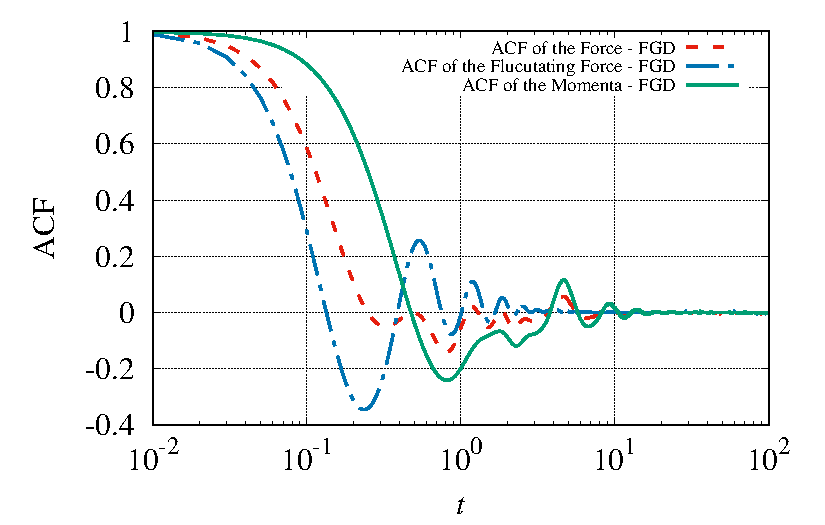
\includegraphics[width=\textwidth]{ACF_comparison}
 \caption{Comparison of the Time Autocorrelation Functions (ACF) between the fluctuating force (purple dot-dashed line), \textit{i.e.} the ``orthogonal'' component of the force, and the momenta (green solid line), in the \emph{Fine-Grained Dynamics} (FGD). All calculations refer to the system C (see table \ref{Tab:Cases}) and are averaged in time and over all beads.}
 \label{Fig:ACFcomparison}
\end{figure}
We can see how there is a separation of the time scales, but it is not as marked and clear  as in the work of Hij\'on \textit{et al.}~\cite{Hijon2006}, being less than one order of magnitude far apart.
Remarkably, this result does not seem to fully justify the Markovian approximation.

As mentioned above, we have studied a system very similar to the one studied by Hij\'on \textit{et al.}~\cite{Hijon2006}. A possible explanation for the lack of separation of scales is that the system analysed here is much smaller than the system studied by them, and that the size of the beads (\textit{i.e.}, the number of atoms in the beads) is much smaller than what they have considered.

\vspace{0.3cm}
For the sake of completeness, we also report in fig.~\ref{Fig:ACF} the ACF for the moments and the forces for the different dynamics, relative to the system C.
\begin{figure}[!htb]
 \begin{subfigure}[b]{0.9\textwidth}
  \centering
   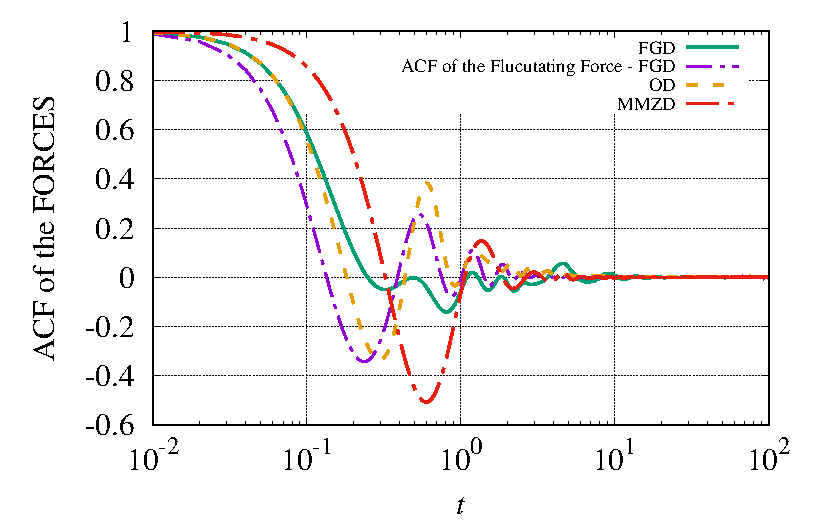
\includegraphics[width=0.9\textwidth]{ACF_F_CORRETTA}
   \caption{The time autocorrelation functions (ACF) of the forces in \emph{Fine-Grained Dynamics} (FGD, green solid line) is compared with its ``orthogonal'' component (Fluctuating Force, purple dot-dashed line) and with the ACF of the forces in \emph{Orthogonal Dynamics} (OD, orange dashed line) and in \emph{Markovian Mori-Zwanzig Dynamics} (MMZD, red dot-dashed line).}
 \end{subfigure}\\
 \begin{subfigure}[b]{0.9\textwidth}
  \centering
  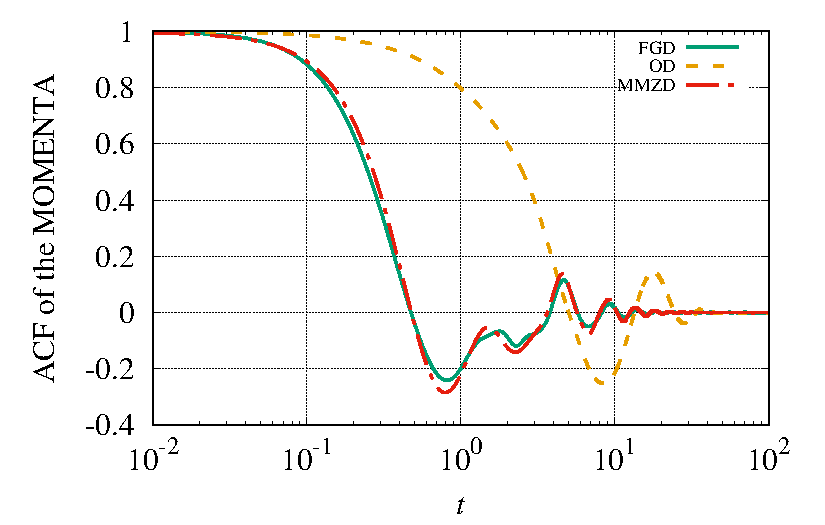
\includegraphics[width=0.9\textwidth]{ACF_P_CORRETTA}
  \caption{The ACF of the momenta in the FGD (green solid line) is compared with the ACF of the momenta in the OD (orange dashed line) and the ACF of the momenta in the MMZD (red dot-dashed line).}
 \end{subfigure}\\
 \caption{Time autocorrelation functions (ACF) of forces and momenta. All calculations refer to the system C (see table \ref{Tab:Cases}) and are averaged in time and over all beads.}
\label{Fig:ACF}
\end{figure}
We can notice how the separation of the time scales is more evident in the case of the orthogonal dynamics, that is, the constrained Hamiltonian dynamics (see Section \ref{Sec:OD}).



\subsection{The effect of the memory approximation on the observables of the studied system}
\label{Sec:Observables}

We compare the observables of the considered system, determined by means of the trajectories of the MMZD and of the CGD, using as target the observables determined by the trajectories of the FGD or using the known theoretical trend, where possible. 
The observables chosen for comparison are
\begin{itemize}
\item[-] linear spatial statistics: the momenta distribution of a single bead and the distribution of inter-bead distance;
\item[-] a dynamics property of the system: the evolution of the mean-square displacement (MSD) of a single bead and of inter-bead distance over time.
\end{itemize}
We would expect that the results of the first observables to be consistent with the reference results determined by the FGD, and in the case of the momenta distribution are consistent with the theoretical trend determined by the Maxwell-Boltzmann distribution. 
While from the results of the MSD we would expect an initial trend with non-trivial differences for the various dynamics and subsequently for long times we would expect a plateau since at long times the beads should oscillate around the equilibrium positions with the same amplitude, regardless of the dynamics employed.

In fig.~\ref{Fig:PDF} we show the distribution of the momenta and inter-bead distance obtained through simulation of FGD, CGD and MMZD, for the system C (see table \ref{Tab:Cases}).
%
\begin{figure}[!htb]
 \begin{subfigure}[b]{0.9\textwidth}
  \centering
   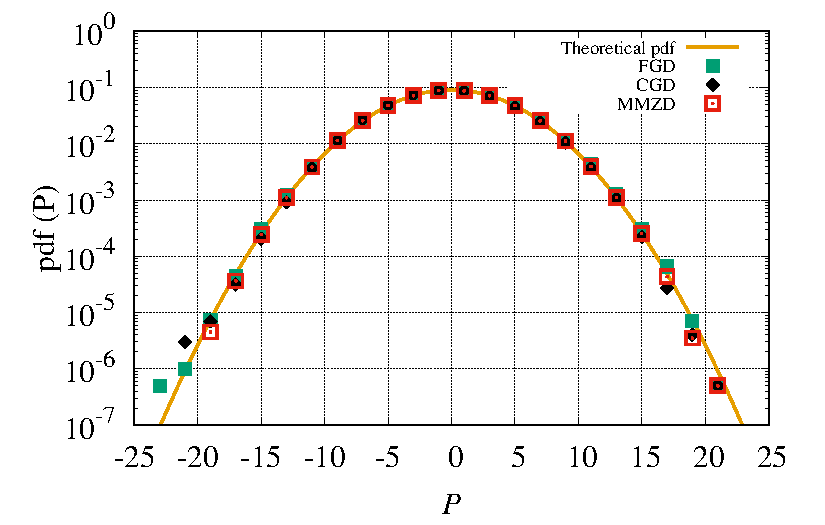
\includegraphics[width=0.9\textwidth]{HistPDF_P_CORRETTAmd}
 \end{subfigure}\\
 \begin{subfigure}[b]{0.9\textwidth}
  \centering
  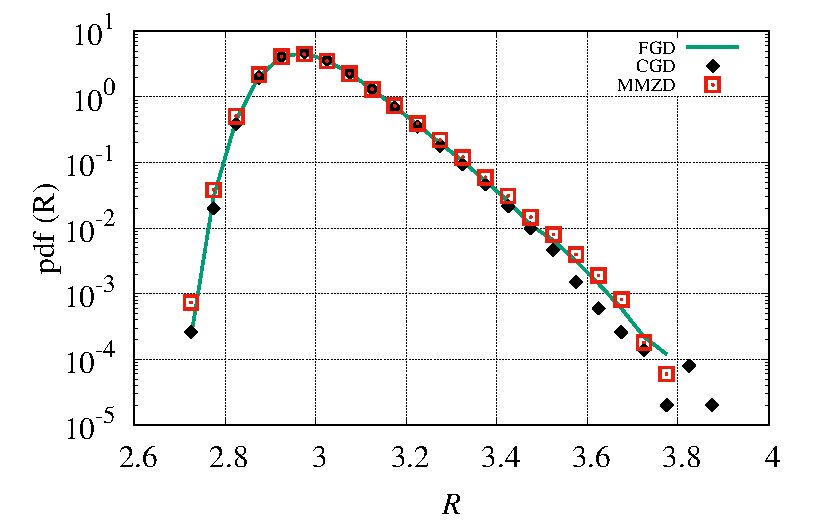
\includegraphics[width=0.9\textwidth]{HistPDF_Q_CORRETTAmd}
 \end{subfigure}\\
 \caption{Comparison of the Probability Distribution Functions (PDFs) of bead momenta (upper panel) and inter-bead distances (bottom panel), between the \emph{Fine-Grained Dynamics} (FGD, green square points and green solid line, respectively), the \emph{Coarse-Grained Dynamics} (CGD, black rhombus points), and the \emph{Markovian Mori-Zwanzig Dynamics} (MMZD, red square points). In the upper panel the simulation results are compared with the expected theoretical trend (orange solid line), \textit{i.e.}, they are compared with the Maxwell-Boltzmann distribution. All calculations refer to system C (see table \ref{Tab:Cases}).}
\label{Fig:PDF}
\end{figure}
%
The distributions of the momenta are the same for all the three systems, and small differences, due to sampling, are visible only in the tails.
%
In the case of the inter-bead distance, the mean value of the inter-bead distance is equal to 2.98 in all three cases, and the bulk of the three distributions overlap completely in the range $2.78\leq R \leq 3.43$. However, there is a systematic difference between the distributions of the CGD and of the other two systems in the right-most tail, with the former being lower. We tentatively ascribe this difference to sampling issues.

A remarkable result obtained is that, thanks to the formalism of MZ, we have obtained a CG model that reproduces the static distributions of the atomistic system without requiring any optimization of the CG potential, as for example happens with the Iterative Boltzmann Inversion (IBI) method \cite{Reith2003}, where the CG potentials are based on the radial distribution functions and are optimized through a series of iterations to recover the correct distribution.   

In fig.~\ref{Fig:MSD} we show the mean-square displacement (MSD) of a single bead over time for the FGD, CGD and MMZD, for the system C (see table \ref{Tab:Cases}).
%
\begin{figure}[!htb]
 \centering
 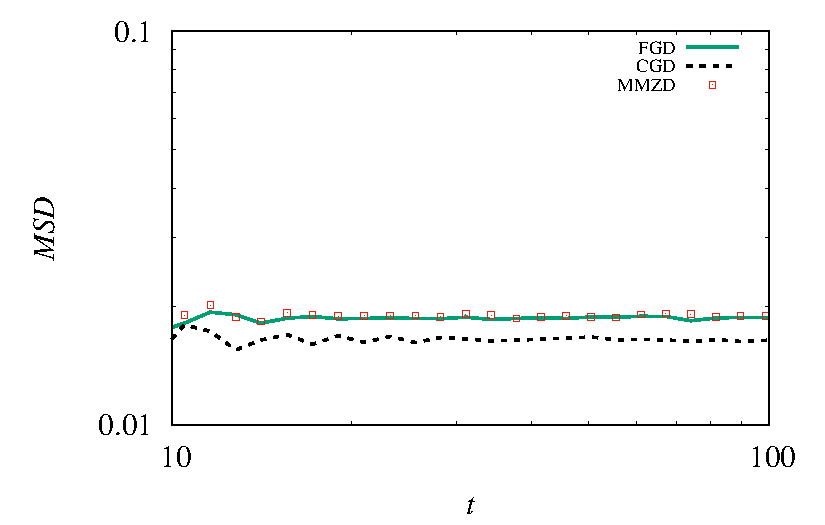
\includegraphics[width=0.9\textwidth]{MSD_CORRETTAmd}
 \caption{Comparison of the Mean Square Displacement (MSD) of a single bead between the \emph{Fine-Grained Dynamics} (FGD, green solid line), the \emph{Coarse-Grained Dynamics} (CGD, black dashed line), and the \emph{Markovian Mori-Zwanzig Dynamics} (MMZD, red square points). All calculations refer to system C (see table \ref{Tab:Cases}) and are averaged in time and over all beads.}
 \label{Fig:MSD}
\end{figure}
%
We can see a first diffusive trend for $t<0.7$, where the FGD and the CGD have the same trend since both have the same thermal bath. While there are small differences between the three systems in this regime, the overall agreement is good.
%
In the time interval $0.7 \leq t \leq 11$, we can see fluctuations of the MSD, which are damped by the coupling to the thermal bath if compared with the results obtained in the $NVE$ case~\cite{DiPasquale2019}. Quite remarkable, the MMZD dynamics is able to correctly capture all the fluctuations, whereas in the CGD system these are slightly out-of-phase.
%
Finally for long time values, we can see that the MSD reaches a plateau. This value is a static property of the system, since at long time values the beads should oscillate around the equilibrium positions with same amplitude. We have already seen in fig.~\ref{Fig:PDF} that the value of the equilibrium position is the same for all dynamics. As a consequence, from the computation of the MSD we should expect the same values of the plateau. However, as we can see in fig.~\ref{Fig:MSD} only the MMZD reaches the value of the reference plateau given by the FGD. The difference value of the plateau of the CGD system is most likely due to the difference in the tails of the distributions of the inter-bead distance discussed above (fig.~\ref{Fig:PDF}). 

\noindent
The deviation of the MSD of the CGD from the reference value may be justified by the difference in the tails of the distributions of the inter-bead distance discussed above (fig.~\ref{Fig:PDF}). 

We observe a qualitatively similar result for the MSD of the inter-bead distance, shown in fig.~\ref{Fig:MSDint}.
%
\begin{figure}[!htb]
 \centering
 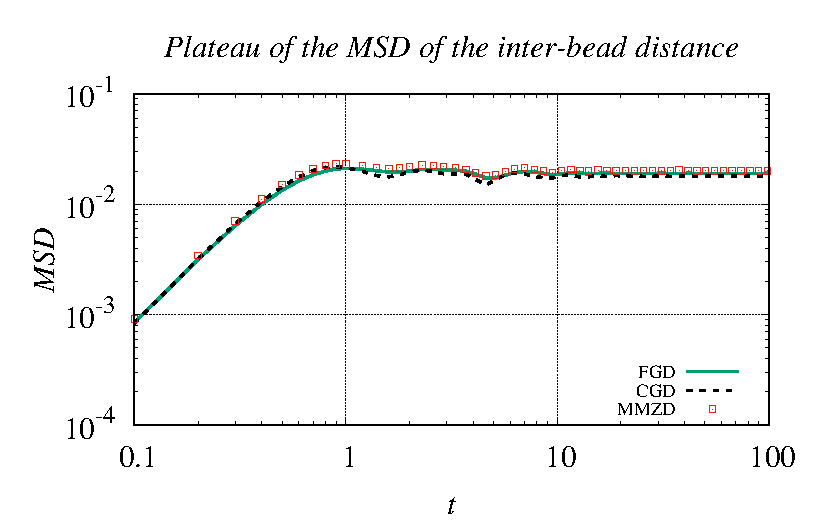
\includegraphics[width=0.9\textwidth]{INT_MSD_CORRETTAmd}
 \caption{Comparison of the Mean Square Displacement (MSD) of the inter-bead distance between the \emph{Fine-Grained Dynamics} (FGD, green solid line), the \emph{Coarse-Grained Dynamics} (CGD, black dashed line), and the \emph{Markovian Mori-Zwanzig Dynamics} (MMZD, red square points). All calculations refer to system C (see table \ref{Tab:Cases}) and are averaged in time and over all beads.}
 \label{Fig:MSDint}
\end{figure}
%
The MMZD system has a behaviour that is closer to the FGD one with respect to the CGD, although the agreement here worsens. Indeed, the oscillations between the MMZD and the FGD are still in phase, but their amplitudes are slightly different, as are the values of the plateau. The CGD fares worse, as in the case MSD case. While the differences in the short-time part of the dynamical observables are due to the approximations considered here, the (small) difference in the long-time behaviour is more puzzling and will require additional work to be properly understood. 

All in all, the results obtained for the CGD and MMZD systems confirm those obtained by Hij\'on \textit{et al.} in Ref.~\cite{ResponseCommentHijon} for a larger system: the behaviour of the CG variables in a system with a non linear potential, such as the L-J potential, is described rather well under the Markovian assumption.


\chapter*{Conclusions}
\phantomsection
\addcontentsline{toc}{chapter}{Conclusions}
\markboth{\MakeUppercase{Conclusions}}{\MakeUppercase{Conclusions}}

In this thesis, we presented the Mori-Zwanzig (MZ) formalism and we gave a rigorous and detailed derivation of the generalized Langevin equation (GLE) for a system in or close to equilibrium, which describes a particle subject to a potential and coupled to a general thermal bath in which memory effects are, in general, present. 
%
Then, through this formalism we derived a class of coarse-grained (CG) models, the so-called hybrid models, that can be used to decrease the computational effort required to simulate generic systems. Subsequently, we studied the integrators needed to implement the numerical simulations in the canonical (NVT) ensemble. Finally, we have numerically studied a toy model, which allowed us to illustrate some of the features of the MZ derivation. 

\noindent
In order to do this we extended and improved a parallel open-source code written in Julia, which we have used to perform simulations of four different systems with different parameters and using different dynamics: the fine-grained dynamics (FGD), the orthogonal dynamics (or constrained dynamics, OD), the  coarse-grained dynamics (CGD) and the Markovian Mori-Zwanzig dynamics (MMZD). Importantly, the sampling of the orthogonal dynamics makes it possible to compute the effective potential and the friction matrix, as well as the fluctuating terms, that enter into the equations of motion derived with the MZ formalism.

In all cases simulated to sample the effective potential, we obtained consistent results with the ones obtained by Di Pasquale \textit{et al.}~in the microcanonical (NVE) ensemble and we note from the figures in Chap.~\ref{Sec:EP} that the coupling to the thermal bath considered here yields curves with a much smaller noise than those obtained in their work. In addition the figures shows how these simple systems have a dependence of fluctuations on the inter-bead distance.

We said in Chap.~\ref{Sec:MarkovApprox} that the validity of the Markovian approximation requires a clear separation of the time scales of the CG system under examination. From the time autocorrelation functions (ACFs) calculated in Section \ref{Sec:ValidAppMARK} we can see how there is a separation of the time scales between the relevant variables and the decay of the memory matrix, but this separation is less than an order of magnitude over a time interval. This result and the fact that the system have a dependence of fluctuations on the inter-bead distance do not seem to fully justify the Markovian approximation.

Remarkably in Sec.~\ref{Sec:Observables}, the observables, both static and dynamic, of the FGD system are reproduced quite well both by the CGD with a simple thermal bath with constant parameters, and by the MMZD with a thermal bath dependent on the inter-bead position. The difference of the statical observables are ascribe to sampling issues. While the differences in the short-time part of the dynamical observables are due to the approximations considered here, instead  the (small) difference in the long-time behaviour is more puzzling and will require additional work to be properly understood.

We wan to stress here that, thanks to the formalism of MZ, we have obtained a CG model that reproduces the static distributions of the atomistic system without requiring any optimization of the CG potential (see the Iterative Boltzmann Inversion (IBI) method, Ref.~\cite{Reith2003}) and without scaling the dynamic quantities obtained by CG simulations by a suitable parameter that measure how faster the CG dynamics is with respect the underlying FG system \cite{Fritz2009}.

The results presented here, which are based on the system studied in Ref.~\cite{DiPasquale2019}, will require additional simulations to evaluate the effect of the size of the system and of the beads considered. Possible future developments of this work are the extension of the code to study systems in two and three spatial dimensions, the evaluation of the transferability of the derived CG model and the development of a better approximation for the memory kernel.


\begin{appendices}

\chapter{Elements of Probability Theory}
\label{App:A}
We introduce some basic definition and results from probability theory. This material can be found in \cite{Williams1991}. 

\begin{defin}[\textbf{Sample Space}]
The set of all events, such as all the possible outcomes of an experiment, is called sample space and is denoted by $\Omega$.  
\end{defin}

\begin{defin}[\textbf{$\sigma$-algebra}]
A collection $\mathscr{F}$ of subset of $\Omega$ is called $\sigma$-algebra on $\Omega$ if\footnote{We use `$\coloneqq$' to signify `is defined to equal', and the following convention:
$$\mathbb{N}\coloneqq\{1,2,3,\dots\} \subseteq \{0,1,2,3,\dots\}\eqqcolon\mathbb{Z}^+\quad\mathrm{and}\quad\mathbb{R}^+\coloneqq[0,+\infty)\,. $$}
\begin{compactenum}[(i)] 
\item $\Omega\in\mathscr{F}$; 
\item $F\in\mathscr{F}\,\implies\, F^c\coloneqq\,\Omega\setminus F\in\mathscr{F}$;
\item $F_n\in\mathscr{F},\,n\in\mathbb{N}\,\implies\,\bigcup_{n\in\mathbb{N}}F_n\in\mathscr{F}$.
\end{compactenum}   
\end{defin}
\noindent
Intuitively, the $\sigma$-algebra $\mathscr{F}$ contains all the useful information that is available about the random experiment that we are performing. One of its elements is called a $\mathscr{F}$-measurable subset of $\Omega$ or \textit{event}.

\begin{defin}[\textbf{Measurable Space}]
A pair $(\Omega,\mathscr{F})$, where $\Omega$ is a set and $\mathscr{F}$ is a $\sigma$-algebra on $\Omega$, is called measurable space.
\end{defin}

\begin{defin}[\textbf{Probability Measure}]
A probability measure $\mathbb{P}$ on the measurable space $(\Omega,\mathscr{F})$ is a function
\[
\mathbb{P}\colon\mathscr{F} \to [0,1];\: F \mapsto \mathbb{P}(F);
\]
satisfying
\begin{compactenum}[(i)] 
\item $\mathbb{P}(\Omega)=1$; 
\item if $F_n\in\mathscr{F}$ with $F_n\bigcap F_m=\emptyset$, $n\neq m$ and $n,m\in\mathbb{N},$ then 
\[ \mathbb{P}\left(\bigcup_{n\in\mathbb{N}}F_n\right)=\sum_{n\in\mathbb{N}}\mathbb{P}\left(F_n\right)\,.\].
\end{compactenum}
\end{defin}

\begin{defin}[\textbf{Probability Space}]
A probability space is a triple $(\Omega,\mathscr{F},\mathbb{P})$ comprising a set $\Omega$, a $\sigma$-algebra $\mathscr{F}$ of subsets of $\Omega$ and a probability measure $\mathbb{P}$ on the measurable space $(\Omega,\mathscr{F})$.
\end{defin}

\noindent
Since we are usually interested in the consequence of the outcomes of an experiment, we introduce the notion of random variable that is intuitively a function of the outcomes. We do it following the Williams \cite{Williams1991}, through the definition of measurable function from $(\Omega,\mathscr{F},\mathbb{P})$ to $(\mathbb{R},\mathscr{B}(\mathbb{R}))$\footnote{We will use the notation $\mathscr{B}(\mathbb{R})$ to denote the Borel $\sigma$-algebra of $\mathbb{R}$, the smallest $\sigma$-algebra containing all open sets of $\mathbb{R}$.}. 

\begin{defin}[\textbf{$\mathscr{F}$-measurable function}]
Let $(\Omega,\mathscr{F},\mathbb{P})$ and $(\mathbb{R},\mathscr{B}(\mathbb{R}))$ be two measurable spaces. 
The function $\psi\colon \Omega\to\mathbb{R}$ is called $\mathscr{F}$-measurable function if 
\[
\psi^{-1}(B)\coloneqq\{\omega\in\Omega\colon \psi(\omega)\in B \}\in\mathscr{F},\quad\forall\, B\in\mathscr{B}(\mathbb{R})\,.
\]
\end{defin}

\begin{defin}[\textbf{Random Variable}]\label{Def:rv}
Let $(\Omega,\mathscr{F},\mathbb{P})$ be a probability space. A random variable is a $\mathscr{F}$-measurable function, thus
\[
X\colon \Omega \to\mathbb{R}\,,\quad X^{-1}\colon \mathscr{B}(\mathbb{R})\to\mathscr{F}\,.
\]
\end{defin}

\noindent
Every random variable, carried by some probability triple $(\Omega,\mathscr{F},\mathbb{P})$, induces a probability measure $\mathbb{P}_X$ on $(\mathbb{R},\mathscr{B}(\mathbb{R}))$:
\begin{align*}
\mathbb{P}_X\colon \mathscr{B}(\mathbb{R}) &\to [0,1] \\
B &\mapsto \mathbb{P}_X(B)\coloneqq\mathbb{P}(X\in B)=\mathbb{P}(X^{-1}(B))\,.
\end{align*}
The measure $\mathbb{P}_X$ is called \emph{distribution} (or sometimes the \emph{law}) of $X$.
We can now define the \emph{distribution function} of $X$:
\begin{align*}
F_X\colon \mathbb{R} &\to[0,1] \\ 
x &\mapsto F_X(x) \coloneqq \mathbb{P}\left( \left\lbrace \omega\in\Omega\colon X(\omega)\leq x \right\rbrace \right)=\mathbb{P}\left( X\leq x\right)\,.
\end{align*}
This function $F_X$ indicates the likelihood that the random variable $X$ is in $(-\infty,x]$.

\begin{defin}[\textbf{Probability density function}]
Let $X$ a random variable and $f:\mathbb{R}\to\mathbb{R}$ a function such that 
\[ f(x)\geq 0 \quad\forall\; x\in\mathbb{R} \qquad\mathrm{and}\qquad \int_{\mathbb{R}	}f(x)\,\mbox{d}x=1\,.\]
We say that $X$ has a \emph{probability density function} (pdf) $f_X$ if 
\[ \mathbb{P}\cip{X\in B}=\int_Bf_X(x)\,\mbox{d}x \qquad \forall\; B\in\mathscr{B}(\mathbb{R}) \]
\end{defin}

\begin{defin}[\textbf{Expected value}]\label{Def:E[...]}
Let $\mathcal{L}^1\cip{\Omega,\mathscr{F},\mathbb{P}}$ be the space of integrable function, see \cite[p. 54]{Williams1991}.
We define the \emph{expectation} $\mathbb{E}\sqp{X}$ of a random variable $X\in \mathcal{L}^1\cip{\Omega,\mathscr{F},\mathbb{P}}$ by 
\begin{equation*} 
\mathbb{E}\sqp{X}\coloneqq \int_{\Omega}X\,\mbox{d}\mathbb{P} \equiv \int_{\Omega}X(\omega)\,\mathbb{P}(\diff\omega) = \int_{\mathbb{R}}x\,\mathbb{P}_X(\diff x)\,, 
\end{equation*}
In the last equality we changed variable $x=X(\omega)$ and used the definition of distribution of $X$, that is $\mathbb{P}_X(B)=\mathbb{P}(X^{-1}(B))$.
\end{defin}

\begin{prop}
Let $h:\mathbb{R}\to\mathbb{R}$ a Borel measurable function and $X\in \mathcal{L}^1\cip{\Omega,\mathscr{F},\mathbb{P}}$ a random variable.

\noindent  
Then $ h(X)\in\mathcal{L}^1\cip{\Omega,\mathscr{F},\mathbb{P}}$ if and only if $h\in\mathcal{L}^1\cip{\Omega,\mathscr{B},\mathbb{P}_X}$
and then
$$\mathbb{E}\sqp{h(X)}=\int_{\mathbb{R}}h(x)\,\mathbb{P}_X(\diff x)\,.$$
Furthermore, if $f_X$ is a pdf of $X$ and
\[
\mathbb{E}\sqp{|h(X)|}<\infty\;\iff\;\int_{\mathbb{R}}|h(x)|\,f_X(x)\,\diff x<\infty\,,
\] 
then
\[
\mathbb{E}\sqp{h(X)}=\int_{\mathbb{R}}h(x)\,f_X(x)\,\diff x\,.
\]
\end{prop}
\begin{proof}
 See Williams \cite[pp.~68-69]{Williams1991}.
\end{proof}

We now give a central definition of modern probability, that is a fundamental theorem (Kolmogorov, 1933).

\begin{theorem}[\textbf{Conditional expectation}]\label{Th:CondExp}
Let $\cip{\Omega,\mathscr{F},\mathbb{P}}$ be a probability space, $X \in \mathcal{L}^1\cip{\Omega,\mathscr{F},\mathbb{P}}$ a random variable and $\mathscr{G}$ a sub-$\sigma$-algebra of $\mathscr{F}$, $\mathscr{G}\subseteq\mathscr{F}$.
Then there exists a random variable $Y\in \mathcal{L}^1\cip{\Omega,\mathscr{G},\mathbb{P}}$, that is $\mathscr{G}$-measurable and $\cexp{\abs{Y}}<\infty$, such that
$$
 \int_G Y\diff\mathbb{P} = \int_G X\diff\mathbb{P}\,,\quad \forall\;G\in\mathscr{G}\,.
$$
Moreover, if $\widetilde{Y}$ is another random variable that has the same properties as $Y$, then $\widetilde{Y}=Y\,a.s.$ (almost surely), i.e. $\mathbb{P}(\widetilde{Y}=Y)=1$.

\noindent
Therefore, $Y$ with these properties is called a \emph{version of the conditional expectation} $\cexpval{X}{\,\mathscr{G}}$ of $X$ given $\mathscr{G}$, and we write $Y=\cexpval{X}{\,\mathscr{G}}\,a.s.$
\end{theorem}
\begin{proof}
 See Williams \cite[pp.~85-86]{Williams1991}.
\end{proof}
\noindent
Generally one identifies several versions and speaks of the conditional expectation $\cexpval{X}{\,\mathscr{G}}$, but we should think about it ``$a.s.$''.

Intuitively, we have already said that the $\sigma$-algebra contains all the useful information that is available on an experiment, while a random variable is a function of its outcomes. In the case the only information we have available regarding which sample point $\omega$ has been chosen is the set of values $Z(\omega)$ for every $\mathscr{G}$-measurable random variable $Z$, i.e. the information available is given by the $\sigma$-algebra generated by $Z$, $\sigma(Z)=\mathscr{G}$. Then the random variable $Y(\omega)=\cexpval{X}{\,\mathscr{G}}(\omega)$ is the expected value of $X(\omega)$ given this information. The ``$a.s.$'' ambiguity in the  definition is something with which, in general, one must live.
 
\begin{defin}[\textbf{Conditional expectation as least-squares-best predictor}]\label{Def:ExpOrthProj}
Let $X \in \mathcal{L}^1\cip{\Omega,\mathscr{F},\mathbb{P}}$ be a random variable such that $\cexp{X^2}<\infty$. Then the conditional expectation $Y=\cexpval{X}{\,\mathscr{G}}$ is a version of the orthogonal projection of $X$ onto $\mathcal{L}^2\cip{\Omega,\mathscr{G},\mathbb{P}}$. 

\noindent
Hence, $Y$ is the least-squares-best $\mathscr{G}$-measurable predictor of $X$: amongst all $\mathscr{G}$-measurable functions, i.e. amongst all predictors which can be computed from the available information, $Y$ minimize $\cexp{\cip{Y-X}^2}$ \cite[p.~85]{Williams1991}. 
\end{defin}
In other words, this definition says that $Y=\cexpval{X}{\,\mathscr{G}}$ is a version of the orthogonal projection of $X\in \mathcal{L}^2\cip{\Omega,\mathscr{F},\mathbb{P}}$ onto $\mathcal{L}^2\cip{\Omega,\mathscr{G},\mathbb{P}}$ if 
$$
 \cexp{\cip{X-Y}^2}\leq\cexp{\cip{X-Z}^2}\,,
$$
$\forall\, Z$ $\mathscr{G}$-measurable such that $\cexp{Z^2}<\infty$.

\noindent 
For a list of properties of the conditional expectation see \cite[p.~88]{Williams1991}. 

\begin{prop}
Let $X,Z\in \mathcal{L}^1\cip{\Omega,\mathscr{F},\mathbb{P}}$ be two random variables which have a \emph{joint probability density function} $f_{X,Z}(x,z)$. 
Then $$f_Z(z)=\int_\real f_{X,Z}(x,z)\diff x$$ acts as pdf for $Z$.

\noindent
Define the \emph{elementary conditional pdf} $f_{X\lvert Z}$ of $X$ given $Z$ via:
$$
f_{X\lvert Z}\cip{x\lvert z} \coloneqq \begin{cases} 
 f_{X,Z}(x,z)/f_Z(z) & \text{if $f_Z(z)\neq 0$ }\,, \\ 
 0 & \text{otherwise}\,.
\end{cases}
$$
Let $h$ be a Borel function on $\real$ such that $\cexp{\abs{h(X)}}<\infty$. Set
$$
g(z) \coloneqq \int_{\real} h(x)f_{X\lvert Z}\cip{x\lvert z}\diff x\,,
$$
then $Y\coloneqq g(Z)$ is a \emph{version of the conditional expectation} of $h(X)$ given $\sigma(Z)$, $\cexpval{h(X)}{\,\sigma(Z)}\equiv\cexpval{h(X)}{\,Z}$.
\end{prop}

\begin{proof}
We can characterize $\sigma(Z)$ as
$$\sigma\cip{Z}=\bp{A=Z^{-1}(B)\,,\;\mathrm{for}\,B\in\mathscr{B}(\real)}\subseteq\mathscr{F}$$ where 
$$Z^{-1}(B)=\bp{\omega\in\Omega\colon Z(\omega)\in B }\in\mathscr{F}\quad\forall\,B\in\mathscr{B}(\real)\,. $$
We introduce the indicator function of $A$ as
$$
I_A(\omega) \coloneqq \begin{cases} 
 1 & \text{if $\omega\in A$}\,, \\ 
 0 & \text{otherwise}\,,
\end{cases}
$$
and from the characterization of $\sigma(Z)$ one has that $I_A(\omega)=I_B(Z)$, since that $\omega \in A$ if and only if $Z(\omega)\in B$.

\noindent
Hence, to show that 
$$
g(Z)=\cexpval{h(X)}{\,Z}=\int_\real h(x) f_{X\lvert Z}\cip{x\lvert z}  \diff x\,
$$
for the theorem (\ref{Th:CondExp}) we must show that
$$
\cexp{g(Z)I_{A}}=\cexp{h(X)I_{A}}\quad\forall\,A\in\sigma(Z)\,.
$$
So we have, applying Fubini's theorem see Ref.~\cite[p.~77-79]{Williams1991},
\begin{multline*}
\cexp{g(Z)I_{A}}=\cexp{g(Z)I_B(Z)} = \int_B g(z)f_Z(z)\,\diff z ={}\\ 
 = \int_{\real} g(z)I_B(z)f_Z(z)\,\diff z =\int_{\real}\cip{\int_\real h(x) f_{X\lvert Z}\cip{x\lvert z}\,\diff x}I_B(z)f_Z(z) \,\diff z ={}\\
   = \int_{\real}\int_{\real} h(x)I_B(z)\,f_{X,Z}(x,z)\,\diff x\,\diff z = \cexp{h(X)I_B(Z)}=\cexp{h(X)I_{A}}\,.
\end{multline*}

\end{proof}


\chapter{Elements of Stochastic Processes}
\label{App:B}
We introduce some basic definition and results from theory of Stochastic Processes. This material can be found in Ref.~\cite{Gardiner2009,Pavliotis2014,Risk:TheFPeq}. 
\section{It\^o Stochastic Differential Equation and the corresponding Fokker-Planck Equation}
\label{Sec:SDE}
An It\^o stochastic differential equation (SDE) can be written as
\[
  \diff \mathbf{x}(t) = \mathbf{a} \sqp{\mathbf{x}(t),t} \diff t+\mathbf{b}\left[\mathbf{x}(t),t\right] \diff \mathbf{W}(t)\,,
\]
where $\mathbf{x}$ are the $n$ stochastic process, $\mathbf{a}(\mathbf{x},t)$ and $\mathbf{b}(\mathbf{x},t)$ are certain know functions, 
$ \diff \mathbf{W}\equiv \boldsymbol{\xi}(t)\,\diff t $ is an $n$ variable Wiener process and $\boldsymbol{\xi}(t)$ is a white noise. This SDE corresponds to a Fokker-Planck equation if the stochastic process described by a conditional probability density $p(\mathbf{x},t\,|\,\mathbf{x_0},t_0)\equiv p$ satisfy 
\[
  \pard{p}{t} = \mathscr{L}(\mathbf{x},t)\,p
     =-\sum_i\,\frac{\partial}{\partial x_i}\left[ A_i(\mathbf{x},t)\,p\, \right]
      +\frac{1}{2}\sum_{ij}\,\frac{\partial^2}{\partial x_i \partial x_j} \left[ B_{ij}(\mathbf{x},t)\,p\, \right] 
\]
where $\mathscr{L}(\mathbf{x},t)$ is a second-order differential operator and the coefficients of RHS are such that $\mathbf{A}(\mathbf{x},t)=\mathbf{a}(\mathbf{x},t)$ and $\underline{\mathbf{B}}(\mathbf{x},t)=\mathbf{b}(\mathbf{x},t)\textbf{b}^T(\mathbf{x},t)$. The Fokker-Planck equation describes diffusion processes, the vector $\mathbf{A}(\mathbf{x},t)$ is known as the drift vector and the matrix $\underline{\mathbf{B}}(\mathbf{x},t)$ is known as the diffusion matrix. From its definition this matrix is positive semidefinite and symmetric \cite{Gardiner2009}.

\subsection{Orstein-Uhlenbeck SDE}
Let us consider an Orstein-Uhlenbeck (OU) SDE, that is, an It\^o equation where the coefficients are
\[
 \mathbf{a}(\mathbf{x})=-k\,\mathbf{x}\quad\text{and}\quad b=\sqrt{D}
\]
here $k$ and $D$ are positive parameters. The solution of one dimensional OU-SDE can be computed by the It\^o's formula applied to $y=xe^{k\,t}$\cite{Gardiner2009}. We get 
\[
 x(t)=x_0(t_0)\,e^{-k(t-t_0)}+\sqrt{D}\int_{t_0}^t\,\diff W(t')e^{-k(t-t')}\,,
\]
and the average and variance are respectively:
\begin{align*}
 \mathbb{E}[x(t)] &= \mathbb{E}[x_0(t_0)]\,e^{-k(t-t_0)}\,, \\
 \mathbb{E}\left[ \left( x(t)-\mathbb{E}[x(t)] \right)^2 \right] &= \left[ Var(x_0)-\frac{D}{2k} \right]e^{-2k(t-t_0)}+\frac{D}{2k}\,.
\end{align*}
We can easily show in the stationary limit ($t\gg t_0$) and applying the equipartition theorem that the diffusive parameter $D$ is equal to $(2k)/\beta$.


\subsection{Langevin Dynamics}
Langevin dynamics combines a conservative dynamic with the OU stochastic vector field as a forcing for the momentum, so we are assuming that the stochastic force is not affected by the potential:
\begin{equation}
\label{Eq:Lang1Dx}
 M \totd{^2x}{t^2} = -\boldsymbol{\nabla} U(\mathbf{x})-\gamma\,\totd{\mathbf{x}}{t}+\sqrt{(2\gamma)/\beta}\,\boldsymbol{\xi}(t)
\end{equation}
where we introduced physical quantities: $M$ is the mass of the particle, $\mathbf{x}$ is the coordinate of position, $\gamma$ is the friction parameter and $\beta=\left( K_BT \right)^{-1}$ is the temperature parameter. We can rewrite the equation as
\[
\begin{cases}
 \diff\mathbf{x}=\mathbf{v}\,\diff t \\
 Md\mathbf{v}=\left[ -\boldsymbol{\nabla} U(\mathbf{x})-\gamma\,\mathbf{v} \right]\,\diff t+\sqrt{(2\gamma)/\beta}\,\diff \mathbf{W}
\end{cases}
\]
and for the canonical coordinates $ \{\mathbf{q}(t),\mathbf{p}(t)\} $ we get 
\begin{equation}
\label{Eq:Lang1Dp}
\begin{cases}
 \diff \mathbf{q} = M^{-1}\,\mathbf{p}\,\diff t \\
 \diff \mathbf{p} = \left[ -\boldsymbol{\nabla} U(\mathbf{q})-\widetilde{\gamma}\,\mathbf{p} \right]\,\diff t
  +\sqrt{(2\widetilde{\gamma})/\beta}\,M^{1/2}\diff \mathbf{W}
\end{cases}
\end{equation}
where $\widetilde{\gamma}=\gamma/M$. From the system of two first-order equations can we compute the drift and diffusion coefficients
\begin{align*}
 \left(A_{\mathbf{q}}\right)_i &= M^{-1}\,p_i\,;  &  \left(B_{\mathbf{q}\mathbf{q}}\right)_{ij} &= \left(B_{\mathbf{p}\mathbf{q}}\right)_{ij}=0\,; \\
 \left(A_{\mathbf{p}}\right)_i &= \left(-\boldsymbol{\nabla} U(\mathbf{q})-\widetilde{\gamma}\,\mathbf{p}\right)_i\,;  &  
      \left(B_{\mathbf{p}\mathbf{p}}\right)_{ij} &= \frac{2\widetilde{\gamma}}{\beta}\,M\,\delta_{ij}\,;
\end{align*}
and thus determine the Fokker-Planck operator for the Langevin dynamics
\begin{multline*}
 \mathscr{L}_{LD}\,\varphi=-M^{-1}\,\sum_i\,p_i\,\partial_{q_i}\,\varphi\,+ 
                          \,\boldsymbol{\nabla}U(\mathbf{q})\,\sum_i\,\partial_{p_i}\,\varphi\,+{}\\                          
                          +\,\widetilde{\gamma}\,\sum_i\,\partial_{p_i}\,p_i\,\varphi\,+
                          \,\widetilde{\gamma}\,\sum_i\,\,p_i\,\partial_{p_i}\,\varphi\,+
                          \,\widetilde{\gamma}\,K_BT\,\sum_i\,M\,\partial_i^2\,\varphi={}\\
                          =-M^{-1}\mathbf{p}\cdot\boldsymbol{\nabla}_{q}\,\varphi\,+
                          \,\boldsymbol{\nabla}U(\mathbf{q})\cdot\boldsymbol{\nabla}_{p}\,\varphi\,+
                          \,\widetilde{\gamma}\, \left[ \,\boldsymbol{\nabla}_{p}(\mathbf{p}\,\varphi)+
                          \,K_BT\boldsymbol{\Delta}_{p}\,\varphi \,\right]\,,
\end{multline*}
where $\boldsymbol{\Delta}_{p}$ is the mass-weighted Laplacian in the momenta and $\varphi$ is a test function \cite{Risk:TheFPeq}.




\chapter{Liouville Space}
\label{App:C}
In classical mechanics, the phase-space\footnote{
Mathematically, the space of configuration might be defined by a \emph{manifold} $M$ (either finite or infinite dimensional), and for each position $\bfr\in M$ in that space, the momentum $\bfp$ of the system would take values in the cotangent space $T^*_{\bfr}M$ of that space. This since the velocity $\dot{\bfr}$ naturally lives in the tangent space $T_{\bfr}M$, but the momentum, for its definition, lives naturally in the cotangent space $T^*_{\bfr}M$:
$$\bfp \coloneqq \pard{L(\bfr,\dot{\bfr})}{\dot{\bfr}},$$ where $L(\bfr,\dot{\bfr})$ is the Lagrangian of the system. 
Therefore the phase-space is naturally represented by the \emph{cotangent bundle} $$T^*M \coloneqq \bp{\cip{\bfr,\bfp}:\;\bfr\in M,\,\bfp\in T^*_{\bfr}M}\,,$$ which comes with a canonical \emph{symplectic form} $\omega\coloneqq \mbox{d}\bfp \wedge \mbox{d}\bfr$.
} 
$X=\mathbb{R}^{6N}$ is the space of all possible states of a physical system composed by N particles. The state is characterized by the instantaneous positions and momenta of the N particles of the system
\begin{equation}\label{gamma}
 \Aphase{}=\cip{ \Aphase{\bfr},\Aphase{\bfp} }=\cip{ \bfr_1,\ldots,\bfr_N , \bfp_1,\ldots,\bfp_N }\,.
\end{equation}
Let $\Ham:X\to \real$ the Hamiltonian of the system and we define a probability measure of finding the system in state $\Aphase{}$ as 
$$
\mathbb{P}(\mbox{d}\Aphase{}) = \rho(\Aphase{})\diff\Aphase{}\,,
$$
where $\rho(\Aphase{})$ can be any equilibrium ensemble pdf. For example, in the canonical ensemble $\rho(\Aphase{})=\partf^{-1}e^{-\beta\Ham(\Aphase{})}$ where $\beta=\cip{K_BT}^{-1}>0$ such that $e^{-\beta\Ham(\Aphase{})}$ is integrable with respect to the Lebesgue measure on $X$ and $\partf$ is the canonical partition function, 
$\partf=\int_Xe^{-\beta\Ham(\Aphase{})}\diff\Aphase{}\,.$

The evolution of a state is obtained in according to the canonical equations of motion as
\begin{equation}
\begin{split}\label{Eq:MotionEq}
  \totd{\Aphase{}}{t} &= \sum_{i=1}^N \sqp{ \pard{\Aphase{}}{\bfr_i} \cdot \dot{\bfr_i}  + \pard{\Aphase{}}{\bfp_i} \cdot \dot{\bfp_i} } ={}\\
               &=\sum_{i=1}^N \sqp{ \pard{\Aphase{}}{\bfr_i} \cdot \pard{\Ham}{\bfp_i} - \pard{\Aphase{}}{\bfp_i} \cdot \pard{\Ham}{\bfr_i} } 
               \equiv \bp{\Aphase{},\Ham}
\end{split}
\end{equation}
where $\bp{\Aphase{},\Ham}$ is Poisson bracket of $\Aphase{}$ with the Hamiltonian $\Ham$. The equation obtained indicates that $\bp{\Aphase{},\Ham}$ is a generator of the time evolution of $\Aphase{}(t)$.

The Poisson bracket allows us to introduce an operator $L$ called \emph{Liouvillian} or \emph{Liouville operator} 
\begin{equation}\label{Eq:liouvilleOperator}
  iL \coloneqq \bp{ \ldots,\Ham} = \sum_{i=1}^N \sqp{ \pard{\Ham}{\bfp_i}\cdot\pard{}{\bfr_i} - \pard{\Ham}{\bfr_i}\cdot\pard{}{\bfp_i} }
\end{equation}
where $i=\sqrt{-1}$.

The equation (\ref{Eq:MotionEq}) can be rewrite as $\mbox{d}\Aphase{}/\mbox{d}t=iL\,\Aphase{}$, which can be formally resolved as
$$
 \Aphase{}(t) = e^{iLt} \,\Aphase{}(0)\,,
$$
where the operator $exp(iLt)$ is know as the \emph{classical propagator} and defines a mapping in phase-space. 

Let $A:X\to\real$ a \emph{phase functions} satisfying $A\in L^2\cip{X,\mathbb{P}}$, where $L^2\cip{X,\mathbb{P}}$ is the Lebesgue space of square-summable functions and where functions are identified if and only if they differ only on a set of measure zero. If $L^2\cip{X,\mathbb{P}}$ comes with the usual scalar product 
\begin{equation}\label{eq:innerProd}
\cip{A,B}=\int_X A(\Aphase{})B(\Aphase{})\, \mathbb{P}(\mbox{d}\Aphase{}) = \int_X A(\Aphase{}) B(\Aphase{})\, \rho(\Aphase{})\,\diff\Aphase{}\,, 
\end{equation}
then $L^2\cip{X,\mathbb{P}}$ is a Hilbert space\footnote{
In general, let $X$ is a set and $\mu$ is a countably additive measure on the $\sigma$-algebra of subsets of $X$. The Hilbert space $L^2\cip{X,\mu}$ is the space of complex-valued measurable functions such that
$$
\int_X|f|^2\diff \mu<\infty,
$$ 
where functions are identified if and only if they differ only on a set of measure zero and where the inner product of a pair of functions $f$, $g$ in $L^2\cip{X,\mu}$ is defined as
$$
\cip{f,g}=\int_Xf^*\,g\,\diff \mu.
$$
}. 
It is simple to show that the rate of change of $A$ is given by $\mbox{d}A/\mbox{d}t=iL\,A$, which formal solution is given by 
\begin{equation}
A(\Aphase{},t) = e^{iLt} \,A(\Aphase{},0)\,.
\end{equation}
The Hilbert space just defined is often called \emph{Liouville space} because the Liouvillian generates the motion in this space. 

In a similar way to quantum mechanics, we can now show that the Liouvillian $L$ is a linear Hermitian operator, that is $L^{\dagger}=L$ where $L^{\dagger}$ is Hermitian conjugate of $L$, and thereby the \emph{classical propagator} is a unitary operator in the phase-space.

We can now define the \emph{time correlation function} $C(t)$ as
\begin{equation}
 C(t) \coloneqq \left\langle A(0)\,A(t)\right\rangle=\int_X A(\Aphase{},0)A(\Aphase{},t)\, \rho(\Aphase{})\diff\Aphase{}\,,
\end{equation}
where $\left\langle\ldots\right\rangle$ denotes an ensemble average. This equation can be expressed as 
\begin{equation*}
C(t) = \int_X A(\Aphase{})\,e^{iLt}A(\Aphase{})\, \rho	(\Aphase{})\diff\Aphase{} = \cip{A(\Aphase{}), e^{iLt}A(\Aphase{}) } = \cip{ A(0),A(t)}\,,
\end{equation*}
thus we obtained
\begin{equation*}
 \left\langle A(0)\,A(t)\right\rangle = \cip{ A(0),A(t)}.
\end{equation*}

\chapter{Dunhamel-Dyson operator identity}
\label{App:D}
The \emph{resolvent} of an operator is define as its Laplace transform. We consider the resolvent of an exponential operator $\exp{At}$:
\begin{multline*}
R_A(s) = \int_0^{\infty} \exp{-st}\exp{-At}\,\diff t = \int_0^{\infty} \exp{-st}\sum_{n=0}^{\infty}\frac{(-At)^n}{n!} \,\diff t ={}\\
   = \sum_{n=0}^{\infty}\frac{(-A)^n}{n!}\int_0^{\infty} \exp{-st}\, t^n\, \diff t =
     \sum_{n=0}^{\infty}\frac{(-A)^n}{n!}\frac{1}{s^{n+1}}\int_0^{\infty} \exp{-st}\, (st)^n\, \diff (st) ={}\\
   = \sum_{n=0}^{\infty}\frac{(-A)^n}{n!}\frac{\Gamma(n+1)}{s^{n+1}} =
     \frac{1}{s}\sum_{n=0}^{\infty}\cip{\frac{-A}{s}}^n = \frac{1}{s}\cip{\idproj+\frac{A}{s}}^{-1} = \cip{s+A}^{-1}, 
\end{multline*}
where we used the definition of gamma function $\Gamma$ and the fact that $\Gamma(n+1)=n!$. 
Therefore, the resolvent of the exponential operator $\exp{-(A+B)\,t}$ is given by 
$$ 
 R_{A,B}(s)=\cip{s+A+B}^{-1}\,.
$$ 
We can rewrite the resolvent obtained through operator identity 
$$
(A+B)^{-1}=A^{-1}-A^{-1}B(A+B)^{-1},
$$
which is easily verified by algebraic manipulations, we are of course assuming invertibility of the relevant operators. So we obtain
$$
 \cip{s+A+B}^{-1}=\cip{s+A}^{-1} - \cip{s+A}^{-1} B\, (s+A+B)^{-1}\,.
$$ 
Substituting the integral representation for the resolvent $R_A(s)$ and for the resolvent $R_{A,B}(s)$ into the equation obtained, we get
\begin{multline*}
 \int_0^{\infty} \exp{-st}\exp{-(A+B)t}\,\diff t ={}\\ 
    = \int_0^{\infty} \exp{-st}\exp{-At}\,\diff t -
      \int_0^{\infty} \exp{-su}\exp{-Au}\,B\,\diff u \int_0^{\infty} \exp{-sv}\exp{-(A+B)v}\,\diff v ={}\\ 
    = \int_0^{\infty} \exp{-st}\exp{-At}\,\diff t - 
      \int_0^{\infty}\exp{-Au}\,B \sqp{ \int_0^{\infty} \exp{-s(u+v)}\exp{-(A+B)v}\,\diff v } \diff u\,.
\end{multline*} 
Keeping $u$ fixed and changing variable $t=u+v$, we can rewrite the internal integral in the equation to obtain
\begin{multline*}
 \int_0^{\infty} \exp{-st}\exp{-(A+B)t}\,\diff t ={}\\ 
  = \int_0^{\infty} \exp{-st}\exp{-At}\,\diff t 
  - \int_0^{\infty}\sqp{ \int_u^{\infty}\exp{-Au}\,B \,\exp{-(A+B)(t-u)}\exp{-st}\,\diff t } \diff u\,.
\end{multline*} 
The region of integration for the double integral is a triangular region in the $(t,u)$ plane and we can reverse the order of integration in the integral to get 
\begin{multline*}
 \int_0^{\infty} \exp{-st}\exp{-(A+B)t}\,\diff t ={}\\ 
   = \int_0^{\infty} \exp{-st}\exp{-At}\,\diff t - 
     \int_0^{\infty}\sqp{ \int_0^{t}\exp{-Au}\,B \,\exp{-(A+B)(t-u)}\diff u } \exp{-st}\,\diff t ={}\\
   = \int_0^{\infty} \exp{-st} \sqp{ \exp{-At}-\int_0^{t}\exp{-Au}\,B\,\exp{-(A+B)(t-u)}\,\diff u }\,\diff t\,. 
\end{multline*}
Since the equality holds for all values of $s$, the integrands must be equal, so:
\begin{equation}\label{Eq:DysId}
 \exp{-(A+B)t} = \exp{-At}-\int_0^{t}\exp{-Au}\,B \,\exp{-(A+B)(t-u)}\,\diff u\,.
\end{equation}
The derivation that we have used here is only valid if both of the operators $A$ and $B$ have no explicit time dependence. 

\noindent
If we consider the operators $\exp{-(A+B)\,t}$ and $\exp{-At}$, then we get
\begin{equation}\label{Eq:IIDysId}
 \exp{(A+B)t} = \exp{At}+\int_0^{t}\exp{Au}\,B \,\exp{(A+B)(t-u)}\,\diff u\,.
\end{equation}
The equations obtained (\ref{Eq:DysId}) and (\ref{Eq:IIDysId}) are the Dyson operator identities, and when applied to propagators they are known as \emph{Dyson decomposition} and \emph{second Dyson decomposition} respectively \cite{evans2008}. 


\end{appendices}

\backmatter

\cleardoublepage
\phantomsection
\addcontentsline{toc}{chapter}{\refname}
\bibliographystyle{plain}
\bibliography{biblioTESI}


\end{document}